% Provenance (never printed): see sources/outline_sources.md (Year 3: primordial
% nucleosynthesis and stellar burning recalled from the physics books; the s and r
% processes; supernovae and neutron-star mergers; galactic chemical evolution; from the
% solar abundances to the composition of the Earth).
% Brief: sources/book5/BRIEFS.md, ch. 30. Curves from figdata/bachelor-3/
% solar_abundances.py (Asplund, Amarsi and Grevesse 2021, Table 2), neutron_capture.py
% (their Table B.1 isotopes, KADoNiS v0.3 cross sections, IAEA Live Chart half-lives) and
% chemical_evolution.py (closed box against the Geneva-Copenhagen survey of Casagrande et
% al. 2011, and a two-phase [alpha/Fe] model). Exercise and problem values in the Book 5
% scratch calculator calc/ch30.py.
\chapter{من أين تأتي العناصر}\label{ch:b3:origin-of-elements}

صُنع الكالسيوم في جرف من الحجر الجيري، في معظمه،
داخل نجوم ضخمة انفجرت قبل أن تولد الشمس. ويأتي حديد لبّ الأرض في معظمه
من نوع مختلف من الانفجار، هو انفجار القزم الأبيض. ويعود بلاتين الخاتم
إلى ذروة في الوفرة بنتها دفعات من \omterm{def:b3:origin-of-elements:s-process}{الأسر النيوتروني} تدوم ثوانٍ،
في اندماج نجمين نيوترونيين أو في نوع نادر من المستعر الأعظم؛
أيُّ الحدثين صنع معظمه ما زال
موضع جدل.
تركت كلٌّ من هذه الأحداث أثرًا في تركيب الشمس،
وهو أيضًا، عدا العناصر القليلة التي لم تستطع الكواكب الاحتفاظ بها، تركيبُ المجموعة الشمسية.
يقرأ هذا الفصل هذا السجلّ: يعرض الوفرات الشمسية،
ويستعيد كيف صُنعت العناصر الخفيفة،
ويتتبّع \omterm{def:b3:origin-of-elements:s-process}{الأسر النيوتروني} الذي بنى العناصر الثقيلة،
ويحدّد المواقع التي تجري فيها كلّ عملية،
ويُنمذج كيف يتغيّر تركيب المجرّة مع حياة نجومها وموتها.
وينتهي حيث تبدأ جيولوجيا المجلدات السابقة: لماذا تكون الأرض،
المصنوعة من المادة نفسها التي صُنعت منها الشمس، غنية جدًّا بالحديد وفقيرة جدًّا في المتطايرات.
% ledger: matteucci21:production, cowan21:rprocess, kobayashi20:origins, asplund21:fig1

\begin{recall}
تخلّق النوى في الانفجار الكبير، واندماج الهيدروجين والهيليوم في النجوم،
وطاقة الربط لكل نوية وذروتها قرب الحديد،
ووادي الاستقرار، والاضمحلال بيتا، وأعمار النصف، والمقطع العرضي لتفاعل،
والنجوم في النسق الأساسي، والعمالقة الحمر، والأقزام البيضاء، والنجوم النيوترونية،
والمستعرات الأعظم، كلّها واردة في كتب الفيزياء. أمّا أصناف النيازك،
وكوندريتات CI، ودرجة حرارة التكاثف، والعناصر المقاومة للحرارة والمتطايرة،
وأصناف غولدشميدت، والأرض السيليكاتية الكلية،
فترد في مجلد السنة الثانية،
في فصوله عن تكوين الكواكب وعن العناصر في الأرض. أمّا بنية درب التبانة،
وقرصيها الرقيق والسميك، وهالتها، وجمهرتها النجمية،
فترد في الفصل السابق.
\end{recall}

\section{الوفرات الشمسية}\label{sec:b3:origin-of-elements:solar}

تحتفظ الشمس بأكثر من \qty{99.85}{\percent} من كتلة المجموعة الشمسية،
وقد احتفظت طبقاتها الخارجية، عدا بعض العناصر الخفيفة وترسّب بطيء لبعض الثقيلة،
بتركيب الغاز الذي تشكّلت منه الشمس والكواكب.
ويُقرأ تركيبها بطريقتين: من خطوط الامتصاص في غلافها الضوئي،
ومن كوندريتات CI، وهي النيازك التي يكون تركيبها،
عدا أشدّ العناصر تطايرًا، هو الأقرب من بين كل المواد المعروفة
إلى تركيب الشمس.
% ledger: asplund21:fig1, asplund21:ci

\begin{definition}[الوفرة الشمسية؛ dex]\label{def:b3:origin-of-elements:abundance}
\emph{الوفرة الشمسية}\index{الوفرة الشمسية} للعنصر $X$ هي
عدد ذراته نسبةً إلى ذرات الهيدروجين في الشمس،
مكتوبًا على مقياس لوغاريتمي يُجعل فيه الهيدروجين عند $12$:
\[
\log\varepsilon(X) = 12 + \log_{10}\frac{N_X}{N_\mathrm{H}} .
\]
والفرق بمقدار وحدة واحدة في مثل هذا اللوغاريتم يُسمّى
\emph{dex}\index{dex}: وفرتان يفصلهما \mbox{\textdir TLT $0.3$~dex} تختلفان بمعامل
قدره $10^{0.3} \approx 2$. أمّا نسبة وفرة عنصر في نجم إلى الشمس
فتُكتب بين أقواس مربعة،
$[X/\mathrm{H}] = \log_{10}(N_X/N_\mathrm{H})_\star -
\log_{10}(N_X/N_\mathrm{H})_\odot$، وبالمثل $[X/Y]$ لأيّ زوج
من العناصر.
\end{definition}

يعرض الشكل أدناه الوفرات الشمسية وفق التجميعة الحديثة
التي أعادت تقييم جميع العناصر الطويلة العمر البالغ عددها 83. أمّا الحديد، فعند
$\log\varepsilon = 7.46$، توجد ذرّة واحدة لكلّ \num{34700} ذرّة من
الهيدروجين؛ ويحتوي الهيليوم على \num{0.0820} ذرّة لكلّ ذرّة هيدروجين. وتبرز عدّة
ملامح، يفسّرها باقي هذا الفصل.
% ledger: asplund21:abstract, asplund21:ci, data:b5-asplund21

\begin{omfigure}
\centering
\begin{tikzpicture}
\begin{axis}[width=0.95\linewidth, height=8.4cm, xmin=0, xmax=94,
  ymin=-1.8, ymax=12.8, xlabel={العدد الذري $Z$},
  ylabel={\mbox{\textdir TLT $\log\varepsilon(X)$ \;($\log\varepsilon(\mathrm{H}) = 12$)}},
  tick label style={font=\scriptsize}, label style={font=\small},
  legend style={font=\scriptsize, at={(0.5,-0.17)}, anchor=north,
    legend columns=2, draw=none, cells={anchor=west},
    /tikz/every even column/.append style={column sep=1em}}]
\addplot[blue!70!black, mark=*, mark size=1.3pt, restrict x to domain=0:84]
  table[x=Z, y=logeps] {figdata/out/bachelor-3-solar_abundances-even.dat};
\addlegendentry{\foreignlanguage{arabic}{\mbox{\textdir TLT $Z$} زوجيّ}}
\addplot[blue!70!black, mark=*, mark size=1.3pt, restrict x to domain=88:94, forget plot]
  table[x=Z, y=logeps] {figdata/out/bachelor-3-solar_abundances-even.dat};
\addplot[red!70!black, mark=o, mark size=1.4pt]
  table[x=Z, y=logeps] {figdata/out/bachelor-3-solar_abundances-odd.dat};
\addlegendentry{\foreignlanguage{arabic}{\mbox{\textdir TLT $Z$} فرديّ}}
\begin{scope}[font=\scriptsize]
\node[anchor=west] at (axis cs:2.2,12.2) {H};
\node[anchor=west] at (axis cs:3.0,10.9) {He};
\node[anchor=west] at (axis cs:5.6,1.0) {Li, Be, B};
\node[anchor=south] at (axis cs:8,8.95) {O};
\node[anchor=south] at (axis cs:6,8.6) {C};
\node[anchor=south, align=center] at (axis cs:26,7.75) {\foreignlanguage{arabic}{\mbox{\textdir TLT Fe}}\\[-1pt]\foreignlanguage{arabic}{ذروة}};
\node[anchor=north] at (axis cs:21,2.95) {Sc};
\node[anchor=south, align=center] at (axis cs:38.5,3.05) {Sr--Zr\\[-1pt]($N = 50$)};
\node[anchor=south] at (axis cs:51.5,2.5) {Te, Xe (r)};
\node[anchor=south, align=center] at (axis cs:58.5,3.7) {Ba\\[-1pt]($N = 82$)};
\node[anchor=south] at (axis cs:76.5,1.95) {Pt (r)};
\node[anchor=south, align=center] at (axis cs:82.5,2.85) {Pb\\[-1pt]($N = 126$)};
\node[anchor=south] at (axis cs:89.6,0.15) {Th};
\node[anchor=north] at (axis cs:92,-0.7) {U};
\end{scope}
\end{axis}
\end{tikzpicture}
\par\smallskip{\small وفرات العناصر في الشمس، على مقياس
لوغاريتمي يكون فيه الهيدروجين عند 12: قيم الغلاف الضوئي، أو قيم
كوندريتات CI للعناصر التي ليس لها خطّ قابل للقياس في الغلاف الضوئي
(أسبلوند، أمارسي وغريسيف، 2021). وتُرسم الأعداد الذرية الزوجية والفردية
بخطّين. لا يملك التكنيشيوم ($Z = 43$) والبروميثيوم ($Z = 61$)
نظيرًا طويل العمر، ولا العناصر الواقعة بين البزموت
والثوريوم.}\label{fig:b3:origin-of-elements:curve}
\end{omfigure}
% ledger: data:b5-asplund21, asplund21:fig1

\begin{enumerate}
\item الهيدروجين والهيليوم يشكّلان تقريبًا كل الذرات، أي ألف مرّة أكثر من جميع العناصر الأخرى مجتمعةً؛
  وقد تكوّن الاثنان في الانفجار الكبير،
  وجزء من الهيليوم منذ ذلك الحين في النجوم.
\item الليثيوم والبريليوم والبورون، التي تلي الهيليوم مباشرةً، تقلّ وفرتها كثيرًا عن الكربون:
  فالبريليوم أقلّ وفرةً بمقدار اثني عشر مليون مرّة.
\item تنخفض الوفرات بحدّة من الأكسجين نحو العناصر الثقيلة، مع قمم حول الأكسجين،
  وحول الحديد، وحول الباريوم، وحول الرصاص،
  وقمم أصغر تُوسَم في الشكل.
\item العناصر ذات العدد الذري الزوجي أوفر من جيرانها الفردية: فالسكانديوم،
  الواقع بين الكالسيوم والتيتانيوم، أندر من الكالسيوم بنحو \num{1400} مرّة،
  وأندر من التيتانيوم بمقدار \num{68} مرّة. وهذا هو
  \emph{تأثير الزوجية والفردية}.
\item بعد قمّة الحديد يتسطّح المنحنى: فمن الحديد إلى الذهب تنخفض الوفرة
  بعامل قدره \num{3.5e6}، لكنّها ترتفع من جديد من الذهب إلى الرصاص
  بعامل قدره أحد عشر.
\end{enumerate}
% ledger: asplund21:fig1, data:b5-asplund21

بالكتلة، يحتوي الغلاف الضوئي الحالي على $X = 0.7438$ من الهيدروجين،
$Y = 0.2423$ من الهيليوم، و$Z = 0.0139$ من كل ما عدا ذلك. وبعد تصحيح أثر العناصر الثقيلة
التي استقرّت تحت الغلاف الضوئي منذ تكوّن الشمس،
فإنّ القيم الأولية للشمس، أي قيم الغاز الذي وُلدت منه الشمس، هي $X = 0.7121$،
و$Y = 0.2725$ و$Z = 0.0154$.
% ledger: asplund21:xyz

\begin{definition}[المعدنية]\label{def:b3:origin-of-elements:metallicity}
\emph{المعدنية}\index{المعدنية} لنجم أو لغاز هي محتواه من
العناصر الأثقل من الهيليوم، والتي تُسمّى معادن في علم الفلك أيًّا كانت كيمياؤها:
وهي تُعطى كنسبة كتلية $Z$، أو، كما يُقاس عادةً،
بوفرة الحديد بالنسبة إلى الشمس، $[\mathrm{Fe/H}]$.
نجم قيمته $[\mathrm{Fe/H}] = -1$ يملك
عُشر ذرّات الحديد لكل ذرّة هيدروجين مما في الشمس.
\end{definition}

يتّفق مصدرا وفرات الشمس اتفاقًا لافتًا.
ويقارن الشكل أدناه بينهما عنصرًا عنصرًا. فبالنسبة إلى 58 عنصرًا،
وهي العناصر التي ليست متطايرة أكثر من اللازم بالنسبة إلى النيازك ولا مدمَّرة في الشمس،
يبلغ المتوسط الموزون للفرق بين وفرة الغلاف الضوئي ووفرة CI
هو $\num[separate-uncertainty=true]{0.000 \pm 0.007}$~\omterm{def:b3:origin-of-elements:abundance}{dex}. وتخرج مجموعتان عن الخط.
فالنيازك تحتوي على كمية أقلّ بكثير من الهيدروجين والهيليوم
والكربون والنيتروجين والأكسجين والغازات النبيلة مقارنةً بالشمس،
إذ بقيت هذه العناصر في الغاز حين تكثّفت المواد الصلبة. وتحتوي الشمس
على ليثيوم أقلّ بمقدار \num{200} مرّة مما في النيازك، إذ دمّرت
\qty{99.5}{\percent} من ليثيومها بالاحتراق النووي.
% ledger: asplund21:ci, data:b5-asplund21

\begin{omfigure}
\centering
\begin{tikzpicture}
\begin{axis}[width=0.66\linewidth, height=0.66\linewidth, xmin=-3, xmax=12.8,
  ymin=-1, ymax=12.8, xlabel={في الكوندريتات \mbox{\textdir TLT CI $\log\varepsilon$}},
  ylabel={في الغلاف الضوئي $\log\varepsilon$},
  tick label style={font=\scriptsize}, label style={font=\small},
  scatter/classes={0={mark=*, mark size=1.3pt, black!70},
    1={mark=square*, mark size=1.5pt, red!70!black},
    2={mark=triangle*, mark size=2pt, blue!70!black}}]
\addplot[black!40, dashed, domain=-1:12.8, samples=2] {x};
\addplot[scatter, only marks, scatter src=explicit symbolic]
  table[x=ci, y=phot, meta=group] {figdata/out/bachelor-3-solar_abundances-compare.dat};
\begin{scope}[font=\scriptsize, red!60!black]
\node[anchor=east] at (axis cs:8.12,12.0) {H};
\node[anchor=west] at (axis cs:1.45,10.914) {He};
\node[anchor=east] at (axis cs:7.25,8.55) {C};
\node[anchor=east] at (axis cs:6.1,7.83) {N};
\node[anchor=west] at (axis cs:8.5,8.45) {O};
\node[anchor=west] at (axis cs:-0.97,8.06) {Ne};
\node[anchor=west] at (axis cs:-0.35,6.38) {Ar};
\node[anchor=west] at (axis cs:-2.12,3.12) {Kr};
\node[anchor=west] at (axis cs:-1.8,2.22) {Xe};
\end{scope}
\node[font=\scriptsize, blue!60!black, anchor=west] at (axis cs:3.4,0.96) {Li};
\end{axis}
\end{tikzpicture}
\par\smallskip{\small الشمس مقابل كوندريتات CI: كل نقطة تمثّل
عنصرًا واحدًا بقيمتيه (أسبلوند، أمارسي وغريسيف، 2021؛ ومقياس النيازك
مضبوط بحيث يتّفق السيليكون). الخطّ المتقطّع يمثّل التساوي. النقاط السوداء:
58 عنصرًا تتّفق قيمها. المربّعات: الهيدروجين والهيليوم والكربون والنيتروجين
والأكسجين والغازات النبيلة، التي لم تحتفظ بها النيازك. المثلّث: الليثيوم،
المدمَّر في
الشمس.}\label{fig:b3:origin-of-elements:sun-ci}
\end{omfigure}
% ledger: data:b5-asplund21, asplund21:ci

الاتفاق حقيقة ذات وزن كبير بالنسبة إلى علم الأرض. ويعني ذلك أنّ
النيازك، التي يمكن تحليلها في المختبر، تعطي تركيب المجموعة الشمسية
لجميع العناصر عدا الأكثر تطايرًا؛ وأنّ الشمس، التي يعطي غلافها الضوئي
الهيدروجين والكربون والنيتروجين والأكسجين، تُكمل ما تبقّى.
وقد بنى مجلد السنة الثانية تركيب الأرض الكلّية
على هذا الأساس.
% ledger: asplund21:ci

\section{العناصر الخفيفة والنجوم}\label{sec:b3:origin-of-elements:stars}

تصف كتب الفيزياء التخليق النووي الأولي في الانفجار الكبير: ففي الدقائق الثلاث الأولى،
ومع برودة الكون، اتّحدت البروتونات والنيوترونات لتكوّن الديوتيريوم،
والهيليوم-3 والهيليوم-4 وأثرًا من الليثيوم-7، ولا إلى عناصر أثقل.
الوفرات الأولية المرصودة هي الكسر الكتلي للهيليوم
$Y_\mathrm{p} = \num[separate-uncertainty=true]{0.245 \pm 0.003}$، ونسبة الديوتيريوم إلى الهيدروجين
\num{2.5e-5}، ونسبة الليثيوم إلى الهيدروجين
\num{1.45e-10}، ويُقاس الأخير في نجوم قديمة فقيرة بالمعادن في هالة المجرّة.
وقد تكوّنت في النجوم كل العناصر الأخرى، وكذلك الفائض من الهيليوم في الشمس،
$0.2725 - 0.245 \approx 0.028$.
% ledger: pdg25:bbn, asplund21:xyz

تحرق النجوم في كتب الفيزياء الهيدروجين إلى هيليوم في النسق الأساسي،
ثم تحرق الهيليوم إلى كربون وأكسجين بوصفها عمالقة حمراء؛ أمّا الأكثر كتلةً فتمضي،
في أغلفة تحيط بلبّها، نحو النيون والمغنيسيوم والسيليكون، وأخيرًا الحديد.
ويتوقّف الاندماج عند هذا الحدّ، لأنّ طاقة الربط لكل نويّة تبلغ أقصاها قرب الحديد:
فبناء نوى أثقل بالاندماج يمتصّ طاقة بدلًا من أن يطلقها.
وبعد قمّة الحديد تُبنى العناصر بطريق آخر هو أسر النيوترونات،
موضوع القسم التالي. أمّا الليثيوم والبريليوم والبورون فهشّة،
إذ تُدمَّر عند درجات الحرارة السائدة في باطن النجوم،
وهو ما جعل الشمس تحرق تقريبًا كل ليثيومها،
وهو أيضًا ما يجعل العناصر الثلاثة
تُشكّل انخفاضًا في منحنى الوفرة.

\begin{definition}[عنصر ألفا]\label{def:b3:origin-of-elements:alpha}
\emph{عنصر ألفا}\index{عنصر ألفا} هو أحد العناصر ذات $Z$ الزوجي
الأكسجين والنيون والمغنيسيوم والسيليكون والكبريت والكالسيوم، والتي
تكون أكثر نظائرها وفرةً ($^{16}\mathrm{O}$، $^{20}\mathrm{Ne}$،
$^{24}\mathrm{Mg}$، $^{28}\mathrm{Si}$، $^{32}\mathrm{S}$،
$^{40}\mathrm{Ca}$) أعدادها الكتلية مضاعفات للعدد أربعة، وهي
تُصنع أساسًا في النجوم الضخمة، وتُعاد إلى الغاز عبر انفجارها
بوصفها مستعرات أعظم ناجمة عن انهيار اللبّ.
\end{definition}
% ledger: matteucci21:production, data:b5-asplund21

إنّ ذروات الأكسجين \omterm{def:b3:origin-of-elements:alpha}{وعناصر ألفا}، وأثر الفردي--الزوجي، هي علامات
على مراحل الحرق هذه: تُدمج نوى الهيليوم في النوى الزوجية أيسر
من دمج أيّ شيء في الفردية، والنوى التي لها عدد زوجي من البروتونات
أشدّ ترابطًا. وما يعيده النجم
إلى الغاز يتوقّف على كتلته.

\begin{definition}[المردود النجمي]\label{def:b3:origin-of-elements:yield}
\emph{المردود النجمي}\index{المردود النجمي} لعنصر ما من نجم ذي كتلة ابتدائية معلومة
هو كتلة ذلك العنصر التي صنعها النجم
حديثًا وأعادها إلى الغاز بين النجوم، عبر الرياح النجمية وفي انفجاره
النهائي، بوصفها كسرًا من كتلة النجم.
\end{definition}
% ledger: matteucci21:yield

النجوم التي تقلّ كتلتها عن \qty{0.8}{M_\odot} تعيش أطول من عمر
الكون ولا تعيد شيئًا. أمّا النجوم التي كتلتها من \num{0.8} إلى \qty{8}{M_\odot}
فتعيد في رياحها الهيليوم والنيتروجين والكربون والعناصر الثقيلة من \omterm{def:b3:origin-of-elements:s-process}{العملية s}
(الباريوم، والإيتريوم، والسترونتيوم) في رياحها، وتنتهي بوصفها أقزامًا بيضاء
من الكربون--الأكسجين. أمّا النجوم التي كتلتها أكبر من \num{8} إلى \qty{10}{M_\odot} فتصنع
أساسًا \omterm{def:b3:origin-of-elements:alpha}{عناصر ألفا} وقدرًا من الحديد، وتنفجر بوصفها مستعرات أعظم ناجمة عن انهيار
اللبّ. ويمكن لقزم أبيض في نظام ثنائي وثيق أن ينفجر بوصفه مستعرًا أعظم من النوع~Ia،
وتُنتج هذه الانفجارات معظم الحديد.
% ledger: matteucci21:production

\begin{omfigure}
\centering
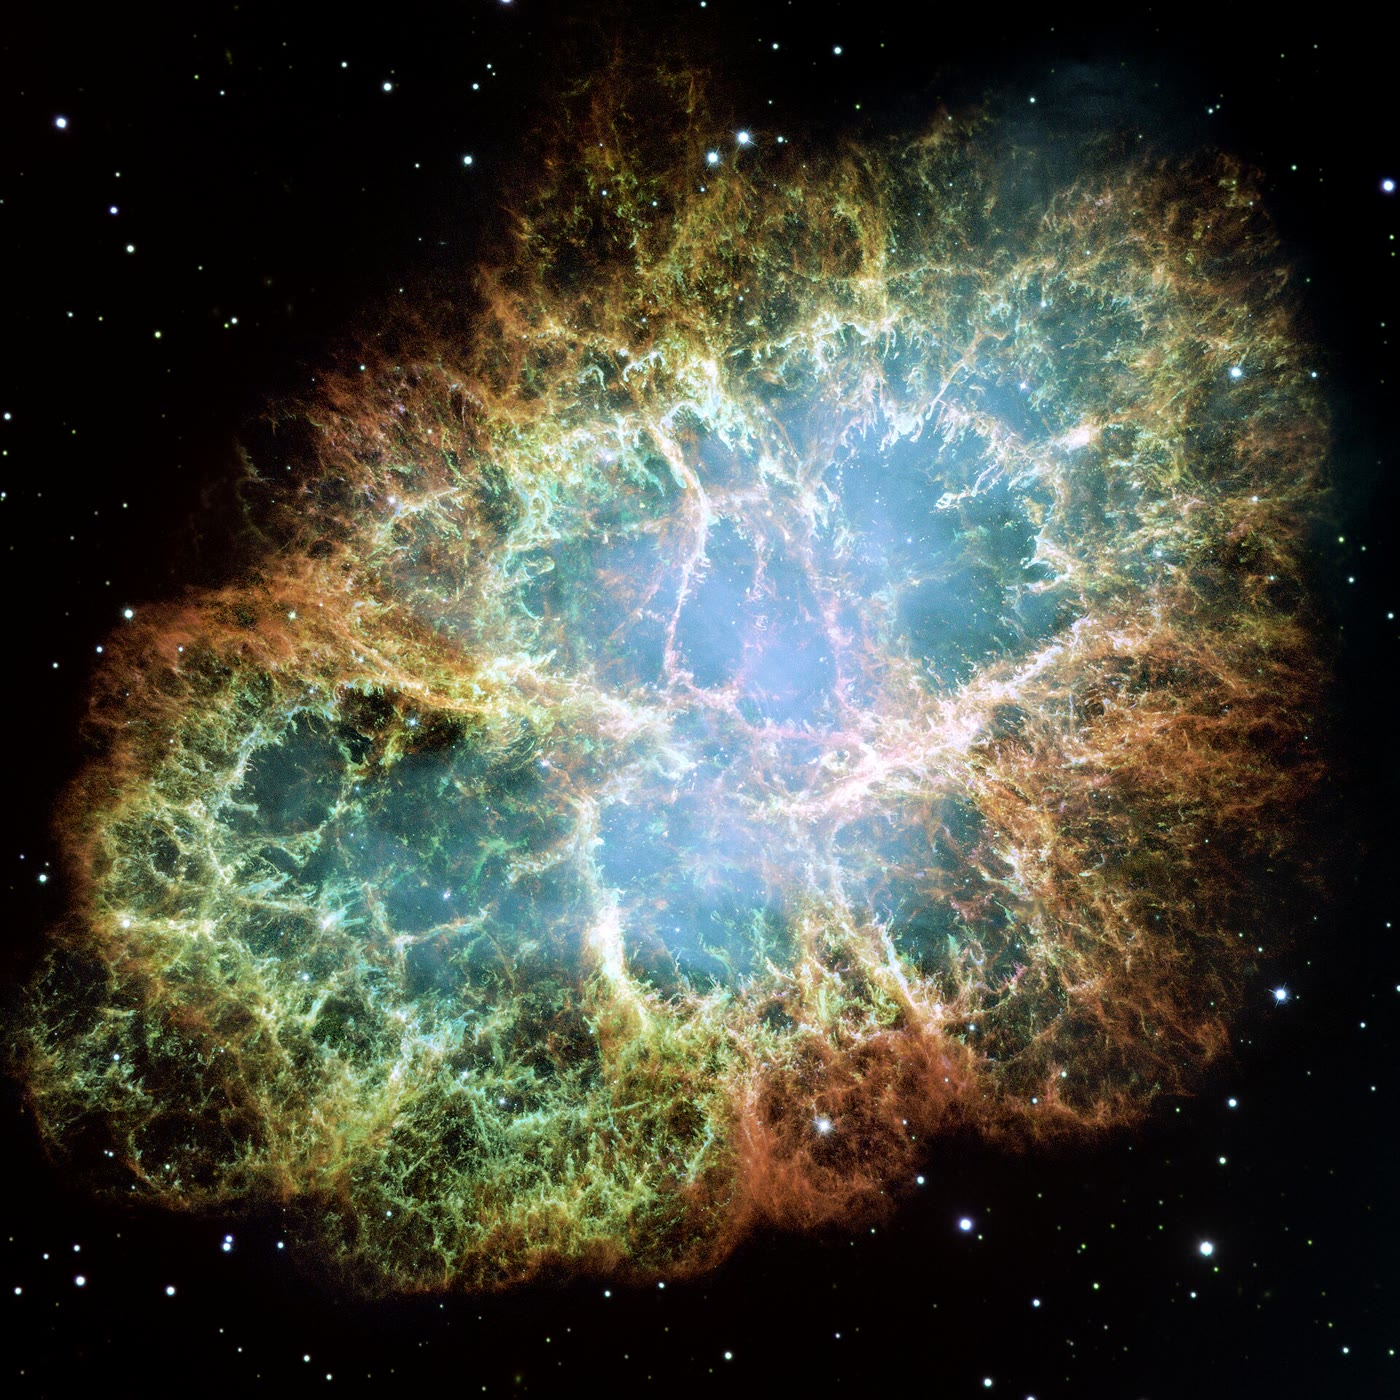
\includegraphics[width=0.5\linewidth]{images/book5/b3-crab-nebula.jpg}
\par\smallskip{\small سديم السرطان، فسيفساء من 24 تعريضًا بتلسكوب هابل الفضائي:
بقايا متمدّدة لنجم انفجاره
سجّله الفلكيون اليابانيون والصينيون عام 1054. والخيوط البرتقالية
هي الطبقات الخارجية الممزّقة للنجم، معظمها هيدروجين؛ أمّا التوهّج المزرق
في الداخل فيأتي من إلكترونات تلتفّ حول خطوط المجال المغنطيسي
للنجم النيوتروني في المركز، الذي يدور ثلاثين مرّة في
الثانية. ويمتزج غاز الخيوط، حاملًا ما صنعه النجم،
بالوسط بين النجوم. \mbox{\textdir TLT NASA, ESA, J.~Hester and A.~Loll}،
ملك عام.}\label{fig:b3:origin-of-elements:crab}
\end{omfigure}
% ledger: photo:b3-crab-nebula

\section{أسر النيوترونات}\label{sec:b3:origin-of-elements:neutrons}

لا يحمل النيوترون شحنة كهربائية، ولا تنفّره النواة: حتّى
النيوترون البطيء يدخل إليها، فتُطلق النواة، وهي أثقل بوحدة كتلة واحدة،
طاقةَ الربط في صورة أشعة غاما. وتُنتج عمليات الأسر المتكرّرة نظائر أثقل
للعنصر نفسه حتى يصبح أحدها غير مستقرّ؛ فيتفكّك عندئذٍ،
عادةً بإصدار بيتا سالبة، إلى العنصر التالي، الذي يأسر
النيوترونات بدوره. وتتوقّف النوى المتكوّنة على مقارنة واحدة: الزمن الفاصل بين
أسرين متتاليين مقارنةً بعمر النصف للنوى غير المستقرّة التي تُصادَف
في الطريق.

\begin{definition}[الأسر النيوتروني؛ العملية s؛ العملية r]\label{def:b3:origin-of-elements:s-process}
\emph{الأسر النيوتروني}\index{الأسر النيوتروني} هو امتصاص نيوترون حرّ
بواسطة نواة، $(Z, A) + \mathrm{n} \to (Z, A+1) + \gamma$.
في \emph{العملية s}\index{العملية s} (البطيئة)، تكون الأسرات
أبطأ من معظم اضمحلالات بيتا: فالزمن بين أسرين متتاليين على النواة الواحدة
يبلغ مئات إلى آلاف السنين، فتضمحل النواة غير المستقرّة في الغالب
قبل أن تأسر، وتتبع سلسلة الأسرات والاضمحلالات
وادي الاستقرار. وفي
\emph{العملية r}\index{العملية r} (السريعة)، تكون كثافة النيوترونات
مرتفعة جدًّا حتى تكون الأسرات أسرع بكثير من الاضمحلالات: فتُدفع النوى
نحو نظائر غنية جدًّا بالنيوترونات، بعيدةً عن الاستقرار، في بضع
ثوانٍ، ثم تضمحل عائدةً إلى الاستقرار متى نفدت النيوترونات.
\end{definition}
% ledger: cowan21:timescales, cowan21:rprocess, kaeppeler11:overview

تصل العمليتان إلى نوى مختلفة، ويُبيّن مخطّط النويدات أيّها.
ويرسم الشكل أدناه شريطًا منه، من الكادميوم إلى الباريوم. وتصعده \omterm{def:b3:origin-of-elements:s-process}{العملية s}
على طول وادي الاستقرار: على امتداد صفّ عنصر ما دامت نظائره مستقرّة،
ثم صعودًا صفًّا واحدًا باضمحلال بيتا.
وتأتي \omterm{def:b3:origin-of-elements:s-process}{العملية r} من الجهة الغنية بالنيوترونات، في الركن السفلي الأيمن:
تضمحل كلّ نواة غنية جدًّا بالنيوترونات باضمحلالات بيتا السالبة المتتالية
على طول متساويها الكتلي، محتفظةً بعددها الكتلي، وتتوقّف عند أوّل
نواة مستقرّة تصادفها. والنواة المستقرّة التي لها متساوٍ مستقرّ
ذو $Z$ أدنى تكون \emph{محمية} من \omterm{def:b3:origin-of-elements:s-process}{العملية r}: $^{122}\mathrm{Te}$
تقع خلف $^{122}\mathrm{Sn}$، و$^{123}\mathrm{Te}$ خلف
$^{123}\mathrm{Sb}$، و$^{124}\mathrm{Te}$ خلف $^{124}\mathrm{Sn}$.
لا يمكن أن تُنتج هذه الثلاث إلّا \omterm{def:b3:origin-of-elements:s-process}{بالعملية s}: فهي
\emph{s فقط}. وعلى العكس، تقع $^{128}\mathrm{Te}$ و$^{130}\mathrm{Te}$
خارج مسار \omterm{def:b3:origin-of-elements:s-process}{العملية s}، وهو ما يترك التيلوريوم عند $^{127}\mathrm{Te}$،
الذي يبلغ عمر نصفه \qty{9.35}{h}: فهي r فقط.
% ledger: kaeppeler11:overview, data:b5-iaea-gs, data:b5-sigman

\begin{omfigure}
\centering
\begin{tikzpicture}
\begin{axis}[x=0.62cm, y=0.7cm, xmin=61.4, xmax=84.6, ymin=47.4, ymax=56.6,
  xlabel={العدد النيوتروني $N$}, ylabel={},
  xtick={62,64,...,84}, ytick={48,...,56},
  yticklabels={Cd 48, In 49, Sn 50, Sb 51, Te 52, I 53, Xe 54, Cs 55, Ba 56},
  tick label style={font=\scriptsize}, label style={font=\small},
  axis line style={black!40}, clip=false,
  scatter/classes={0={mark=square*, mark size=6.5pt, blue!45},
    1={mark=square*, mark size=6.5pt, black!18},
    2={mark=square*, mark size=6.5pt, red!40},
    3={mark=square*, mark size=6.5pt, orange!45}}]
\addplot[only marks, mark=square, mark size=6.5pt, black!45, thin,
  restrict x to domain=61:85]
  table[x=N, y=Z] {figdata/out/bachelor-3-neutron_capture-unstable.dat};
\addplot[scatter, only marks, scatter src=explicit symbolic,
  restrict x to domain=61:85]
  table[x=N, y=Z, meta=cls] {figdata/out/bachelor-3-neutron_capture-chart.dat};
\addplot[only marks, mark=none, nodes near coords={\massnum},
  restrict x to domain=61:85,
  visualization depends on={value \thisrow{A} \as \massnum},
  nodes near coords align={center}, every node near coord/.append style={font=\tiny}]
  table[x=N, y=Z] {figdata/out/bachelor-3-neutron_capture-chart.dat};
\addplot[only marks, mark=none, nodes near coords={\massnum}, restrict x to domain=61:85,
  visualization depends on={value \thisrow{A} \as \massnum},
  nodes near coords align={center}, every node near coord/.append style={font=\tiny, black!55}]
  table[x=N, y=Z] {figdata/out/bachelor-3-neutron_capture-unstable.dat};
\addplot[quiver={u=0.48*\thisrow{dN}, v=0.48*\thisrow{dZ}}, -{Stealth[length=3pt]},
  blue!60!black, semithick, restrict x to domain=61:85]
  table[x expr=\thisrow{N0}+0.26*\thisrow{dN}, y expr=\thisrow{Z0}+0.26*\thisrow{dZ}]
  {figdata/out/bachelor-3-neutron_capture-path.dat};
\begin{scope}[red!70!black, dashed, -{Stealth[length=4pt]}, thick]
\draw (axis cs:79.1,48.9) -- (axis cs:76.4,51.6);
\draw (axis cs:81.1,48.9) -- (axis cs:78.4,51.6);
\draw (axis cs:83.1,50.9) -- (axis cs:80.4,53.6);
\end{scope}
\node[font=\scriptsize, red!70!black, anchor=south east, align=right] at (axis cs:84.5,47.5)
  {\foreignlanguage{arabic}{اضمحلالات العملية r}\\[-1pt]\foreignlanguage{arabic}{على طول المتساويات الكتلية}};
\end{axis}
\end{tikzpicture}
\par\smallskip{\small قطاع من مخطّط النويدات، من الكادميوم
إلى الباريوم، بأعداد نيوترونية من 62 إلى 84. والمربّعات الملوّنة هي النوى الموجودة في الطبيعة،
موسومةً بعددها الكتلي: الأزرق، s فقط؛ والرمادي، تُنتجه العمليتان؛ والأحمر،
r فقط؛ والبرتقالي، نوى p، ولا تبلغها أيّ من العمليتين. والمربّعات المفتوحة هي
النوى غير المستقرّة التي تمرّ بها \omterm{def:b3:origin-of-elements:s-process}{العملية s}. والأسهم الزرقاء: مسار \omterm{def:b3:origin-of-elements:s-process}{العملية s}،
الأسر نحو اليمين، واضمحلالات بيتا قطريًّا نحو الأعلى واليسار (عند
$^{134}\mathrm{Cs}$ و$^{135}\mathrm{Cs}$ يتفرّع المسار). والأسهم الحمراء المتقطّعة
تمثّل ثلاثًا من سلاسل اضمحلال \omterm{def:b3:origin-of-elements:s-process}{العملية r}، تنتهي عند
$^{128}\mathrm{Te}$، و$^{130}\mathrm{Te}$ و$^{134}\mathrm{Xe}$. وتُحسب
الفئات انطلاقًا من النظائر الموجودة في الطبيعة
\babelsublr{(Asplund, Amarsi and Grevesse, 2021)}، وأعمار النصف وأنماط الاضمحلال في
مخطّط النويدات الصادر عن IAEA.}\label{fig:b3:origin-of-elements:chart}
\end{omfigure}
% ledger: data:b5-sigman, data:b5-iaea-gs, data:b5-asplund21, kaeppeler11:branchings

المجموعة الثالثة، وهي المربّعات البرتقالية، لا تبلغها أيّ من العمليتين: النظائر
الغنية بالبروتونات مثل $^{112}\mathrm{Sn}$، $^{120}\mathrm{Te}$
أو $^{124}\mathrm{Xe}$.

\begin{definition}[النوى p]\label{def:b3:origin-of-elements:p-process}
\emph{النوى p}\index{النوى p} هي النظائر المستقرّة
في الجانب الغني بالبروتونات من وادي الاستقرار، بعد ذروة الحديد، والتي
لا تستطيع \omterm{def:b3:origin-of-elements:s-process}{العملية s} ولا \omterm{def:b3:origin-of-elements:s-process}{العملية r} إنتاجها: فهي محمية من \omterm{def:b3:origin-of-elements:s-process}{العملية r}
بنظير مستقرّ متساوٍ في العدد الكتلي وذي $Z$ أدنى، وتقع خارج مسار \omterm{def:b3:origin-of-elements:s-process}{العملية s}.
تُعزى إلى عملية p مستقلّة، يُرجَّح أنّها تحدث في انفجارات المستعرات العظمى،
وباستثناءات قليلة تكون وفرتها أقلّ بكثير من وفرة نظائر s و r
المجاورة لها.
\end{definition}
% ledger: kaeppeler11:overview

تُطبَّق القاعدة التي تقرأ المخطّط على جميع النويدات البالغ عددها 287 في
الجدول ما قبل الشمسي الواقعة بعد الزنك، فتجد 30 نويدةً s فقط و29 نويدةً r فقط
و36 من \omterm{def:b3:origin-of-elements:p-process}{النوى p}. وإحدى هذه \omterm{def:b3:origin-of-elements:p-process}{النوى p}، وهي $^{176}\mathrm{Hf}$، تبلغها في الواقع
\omterm{def:b3:origin-of-elements:s-process}{العملية s} عبر حالة مثارة طويلة العمر في
$^{176}\mathrm{Lu}$ تتجاهلها القاعدة البسيطة؛ أمّا النويدات الأخرى، وعددها 35، فهي \omterm{def:b3:origin-of-elements:p-process}{النوى p}
المعروفة في الأدبيات.
% ledger: data:b5-sigman, kaeppeler11:branchings

يمكن تتبّع \omterm{def:b3:origin-of-elements:s-process}{العملية s} كمّيًّا، لأنّ نويداتها
قريبة من الاستقرار، ويمكن قياس مقاطع أسرها. ففي بلازما نجمية عند درجة الحرارة
$T$ تصبح النيوترونات متوازنة حراريًّا، والمهمّ هو
مقطع الأسر المتوسَّط على توزيع ماكسويل-بولتزمان لها،
$\langle\sigma\rangle$، المُعطى عند طاقة حرارية
$kT = \qty{30}{keV}$.
% ledger: kaeppeler11:classical

\begin{proposition}[علاقة $\sigma N$]\label{prop:b3:origin-of-elements:sigma-n}
\index{علاقة@$\sigma N$ علاقة}
على مقطع من مسار \omterm{def:b3:origin-of-elements:s-process}{العملية s} تكون فيه كلّ نواة مستقرّة، وتكون كثافة
النيوترونات $n_\mathrm{n}$ ودرجة الحرارة ثابتتان، وليكن $N_A$ وفرةَ النواة
ذات العدد الكتلي $A$ و$\langle\sigma\rangle_A$ مقطعها المتوسَّط.
فإذا بلغ تدفّق النيوترونات حالةً مستقرّة،
فإنّ
\[
\langle\sigma\rangle_{A-1} N_{A-1} = \langle\sigma\rangle_A N_A ,
\]
ومنه يكون الجداء $\sigma N$ متساويًا لكلّ نواة
في المقطع.
\end{proposition}

\begin{proof}
تأسر نواةٌ كتلتها $A$ النيوترونات بالمعدّل
$\lambda_A = n_\mathrm{n}\langle\sigma\rangle_A v_T$ لكلّ نواة، حيث
$v_T$ متوسّط السرعة الحرارية للنيوترونات. وتتكوّن النواة بالأسر
على النواة $A - 1$ وتُستهلك بالأسر على نفسها، لذلك
$\mathrm{d}N_A/\mathrm{d}t = n_\mathrm{n} v_T\,(\langle\sigma\rangle_{A-1}
N_{A-1} - \langle\sigma\rangle_A N_A)$. وفي الحالة المستقرّة
يتلاشى المشتقّ، وهو العلاقة المطلوبة. فالنواة ذات المقطع الكبير تُمرَّر
بسرعة وتبقى نادرة؛ أمّا التي مقطعها صغير
فتتراكم.
\end{proof}
% ledger: kaeppeler11:classical

تختبر ذلك النظائرُ الثلاثة s فقط للتيلّوريوم. وتبلغ وفرتها ما قبل الشمسية
\num{0.1067}، \num{0.0373} و\num{0.1984} ذرّةً لكلّ
مليون ذرّة سيليكون، ومقاطع أسرها \num{295}، \num{832}
و\qty{155}{mb}: تبلغ الجداءات \num{31.5}، \num{31.0}
و\qty{30.8}{mb}، متساوية ضمن ثلاثة بالمئة، رغم أنّ الوفرات
تختلف بمعامل قدره خمسة. وعند عدد سحري نيوتروني
تنكسر العلاقة، إذ تكون النوى ذات $N = 50$، $82$ أو $126$ مرتبطةً بشدّة إلى حدّ أنّها
تأسر بضعف، ويبلغ $\langle\sigma\rangle = \qty{4.0}{mb}$ في
$^{138}\mathrm{Ba}$ مقابل \qty{61.2}{mb} في $^{136}\mathrm{Ba}$،
وتعمل كعنق زجاجة. ويبيّن الشكل الآتي الجداء لجميع
النويدات s فقط: هضاب مستوية تفصل بينها قفزات قرب $A = 88$، $140$
و$208$.
% ledger: data:b5-sigman, data:b5-kadonis, kaeppeler11:classical

\begin{omfigure}
\centering
\begin{tikzpicture}
\begin{axis}[width=0.95\linewidth, height=7.4cm, xmin=60, xmax=212,
  ymode=log, ymin=1, ymax=5000, xlabel={العدد الكتلي $A$},
  ylabel={الجداء $\langle\sigma\rangle N$ (mb، لكلّ $10^6$ ذرّة سيليكون)},
  tick label style={font=\scriptsize}, label style={font=\small},
  legend style={font=\scriptsize, at={(0.5,-0.17)}, anchor=north,
    legend columns=2, draw=none, cells={anchor=west},
    /tikz/every even column/.append style={column sep=1em}}]
\draw[black!35, dotted, thick] (axis cs:88,1) -- (axis cs:88,5000);
\draw[black!35, dotted, thick] (axis cs:139,1) -- (axis cs:139,5000);
\draw[black!35, dotted, thick] (axis cs:208,1) -- (axis cs:208,5000);
\addplot[blue!70!black, thick, const plot]
  table[x=A, y=sigN_model] {figdata/out/bachelor-3-neutron_capture-fitted.dat};
\addlegendentry{\foreignlanguage{arabic}{النموذج الكلاسيكي المُطابَق من أجل $A > 90$}}
\addplot[only marks, mark=*, mark size=1.7pt, red!70!black]
  table[x=A, y=sigN] {figdata/out/bachelor-3-neutron_capture-sigman.dat};
\addlegendentry{\foreignlanguage{arabic}{النويدات s فقط}}
\begin{scope}[font=\scriptsize]
\node[anchor=south west] at (axis cs:88.5,1.1) {$N = 50$};
\node[anchor=south west] at (axis cs:139.5,1.1) {$N = 82$};
\node[anchor=south east] at (axis cs:207.5,1.1) {$N = 126$};
\node[anchor=south] at (axis cs:123,38) {Te};
\node[anchor=south] at (axis cs:135,33) {Ba};
\node[anchor=north] at (axis cs:149,6.6) {Sm};
\node[anchor=west] at (axis cs:177,1.79) {Lu};
\node[anchor=west] at (axis cs:71,2326) {Ge};
\node[anchor=west] at (axis cs:83,428) {Kr};
\end{scope}
\end{axis}
\end{tikzpicture}
\par\smallskip{\small جداء مقطع \omterm{def:b3:origin-of-elements:s-process}{الأسر النيوتروني}
عند \qty{30}{keV} \babelsublr{(KADoNiS)} والوفرة ما قبل الشمسية
\babelsublr{(Asplund, Amarsi and Grevesse, 2021)} للنويدات \babelsublr{30 s} فقط. وبين الأعداد السحرية
النيوترونية (الخطوط المنقّطة) يكاد الجداء يكون ثابتًا؛ وعند كلّ منها يُكبح التدفّق
فينخفض الجداء. ويمثّل الخطّ النموذج الكلاسيكي للعملية s
المُطابَق هنا للنويدات الأثقل من $A = 90$. أمّا
الأخفّ فتحتاج إلى مكوّن ثانٍ أضعف،
يتكوّن في النجوم الضخمة.}\label{fig:b3:origin-of-elements:sigma-n}
\end{omfigure}
% ledger: data:b5-sigman, data:b5-kadonis, data:b5-asplund21, kaeppeler11:classical

يمثّل الخطّ في الشكل النموذج الكلاسيكي للعملية s: يُعرَّض جزء صغير
$G$ من الحديد-56 للنيوترونات، مع توزّع التعرّضات أُسّيًّا
حول متوسّط $\tau_0$، ويُتابَع التدفّق نويدةً بعد نويدة
بالمقاطع العرضية المقيسة. ويُطابَق هذا النموذج على \num{22} نويدة مُنتَجة \omterm{def:b3:origin-of-elements:s-process}{بالعملية s} وحدها
والأثقل من $A = 90$ (مع استبعاد $^{176}\mathrm{Lu}$، الذي يتفكّك،
و$^{187}\mathrm{Os}$، الذي يُغذّى بتفكّك
$^{187}\mathrm{Re}$)، فيعطي $\tau_0 = \qty{0.31}{mb^{-1}}$
و$G = \qty{0.054}{\percent}$ من حديد-56 الشمسي، وهي قريبة من
\qty{0.04}{\percent} التي تعطيها التحليلات التفصيلية، حيث تلتقط كلّ نويدة بذرة
في المتوسّط نحو خمس عشرة نيوترونًا. أمّا أخفّ النويدات المُنتَجة \omterm{def:b3:origin-of-elements:s-process}{بالعملية s} وحدها
أي الجرمانيوم-70 والسيلينيوم-76، فتقع بعيدًا فوق الخطّ: إنّها تحتاج إلى
مكوّن ثانٍ ضعيف، يتكوّن في النجوم الضخمة.
% ledger: data:b5-sigman, kaeppeler11:classical

حين تعيش نويدة غير مستقرّة على المسار مدّةً تقارب الزمن الفاصل بين عمليتي أسر متتاليتين، ينقسم التدفّق:
يتفكّك جزء منه، ويلتقط الجزء الآخر نيوترونًا.
وتحدث مثل هذه \emph{التفرّعات} عند $^{79}\mathrm{Se}$، $^{85}\mathrm{Kr}$،
$^{134}\mathrm{Cs}$، $^{147}\mathrm{Pm}$ و$^{151}\mathrm{Sm}$، من بين
غيرها. يتيح التفرّع أن يتجاوز جزء من التدفّق نويدةً بعينها: فمن
نظيري السماريوم المُنتَجين \omterm{def:b3:origin-of-elements:s-process}{بالعملية s} وحدها، يستقبل $^{150}\mathrm{Sm}$ التدفّق كلّه،
بينما لا يستقبل $^{148}\mathrm{Sm}$ إلّا الجزء الذي التفّ حول التفرّع
عند الكتلة 147، ونسبة $\sigma N$ لهما، \num{0.87}،
تقيس ذلك الجزء. ولأنّ هذا الجزء يعتمد على كثافة النيوترونات
ودرجة الحرارة، فإنّ التفرّعات مقاييس حرارة ومقاييس كثافة للنجوم
التي جرت فيها \omterm{def:b3:origin-of-elements:s-process}{العملية s}.
% ledger: kaeppeler11:branchings, kaeppeler11:pairs, data:b5-sigman

\begin{inthelab}[قياس مقطع الأسر العرضي]
لقياس المقاطع العرضية المتوسّطة التي تحتاجها \omterm{def:b3:origin-of-elements:s-process}{العملية s}،
يُعيد الفيزيائيون إنتاج طيف نيوتروني نجمي في مسرّع.
تُصطدم البروتونات بهدف من الليثيوم فتُنتج النيوترونات بالتفاعل
$^{7}\mathrm{Li}(\mathrm{p},\mathrm{n})^{7}\mathrm{Be}$، ويحاكي طيفه
طيفًا حراريًا عند $kT = \qty{25}{keV}$، وهي قيمة قريبة من
\qty{23}{keV} التي تميّز ومضات قشرة الهيليوم في العملاق الأحمر. تُوضَع العيّنة
ملاصقةً للهدف، في أقوى تدفّق، وبعد
التشعيع تُعَدّ أشعّة غاما الصادرة عن النويدات المشعّة المُنتَجة حديثًا:
تعمل طريقة التنشيط هذه بعيّنات تقلّ عن
ميكروغرام واحد. وحين يكون الناتج مستقرًّا، تُرسَل النيوترونات في نبضات
ويُقاس زمن طيرانها على مسار معيّن لتحديد طاقتها، وتسجّل كرة من
بلّورات فلوريد الباريوم المحيطة بالعيّنة تتالي أشعّة غاما
لكلّ أسر.
\end{inthelab}
% ledger: kaeppeler11:lab

\begin{history}[التكنيشيوم في العمالقة الحمراء]
في عام 1952 وجد بي. دبليو. ميريل خطوط التكنيشيوم في أطياف
العمالقة الحمراء من النوع الطيفي S. ليس للتكنيشيوم نظير مستقرّ؛ أمّا النظير
الذي تنتجه \omterm{def:b3:origin-of-elements:s-process}{العملية s}، $^{99}\mathrm{Tc}$، فيبلغ عمر نصفه
\num{211000} سنة، وهو أقصر بكثير من الأعمار التي عاشتها هذه النجوم.
كان لا بدّ أن يكون التكنيشيوم قد تكوّن داخل النجوم، وفي
زمن قريب. كان ذلك أوّل دليل مباشر على أنّ النجوم تُنتج العناصر. وفي
عام 1957 صاغ إي. إم. وجي. آر. بوربيدج، ودبليو. إيه. فاولر، وإف. هويل،
وبشكل مستقلّ إيه. جي. دبليو. كاميرون، النموذج الكلاسيكي
للعملية s.
\end{history}
% ledger: kaeppeler11:overview, data:b5-iaea-gs

تترك \omterm{def:b3:origin-of-elements:s-process}{العملية r} قممها الخاصّة. ويقع مسارها قريبًا من حدّ تسرّب النيوترونات
وهو الحدّ الذي تعجز بعده النويدة عن استبقاء نيوترون إضافي،
ويتوقّف التدفّق عند النويدات ذات الأغلفة النيوترونية المغلقة، $N = 50$، $82$
و$126$، حتّى تتفكّك بيتا. تتراكم المادّة في هذه النقاط المؤقّتة؛
وبعد التفكّكات النهائية نحو الاستقرار تقع الأكوام عند أعداد كتلية أدنى بعدّة
وحدات من قمم \omterm{def:b3:origin-of-elements:s-process}{العملية s} للأعداد السحرية نفسها، وهي
مكوّنة من نويدات مستقرّة: قرب $A = 130$ (التيلوريوم والزينون)
و$A = 195$ (البلاتين)، مقابل $A = 138$ و$208$ لقمم \omterm{def:b3:origin-of-elements:s-process}{العملية s}
للباريوم والرصاص. يُظهر منحنى الوفرة المجموعتين من القمم جنبًا إلى
جنب. تُنتج \omterm{def:b3:origin-of-elements:s-process}{العملية r} نحو نصف العناصر الثقيلة، وتُنتج \omterm{def:b3:origin-of-elements:s-process}{العملية s}
النصف الآخر.
% ledger: cowan21:rprocess, kaeppeler11:overview, kaeppeler11:classical

\section{أين تجري العمليات}\label{sec:b3:origin-of-elements:sites}

تجري \omterm{def:b3:origin-of-elements:s-process}{العملية s} الرئيسية في العمالقة الحمراء التي تبلغ كتلتها حتى نحو ثلاث كتل شمسية،
قرب نهاية عمرها، بوصفها نجومًا على فرع العملاقة المقارِبة. وبين
ومضات احتراق الهيليوم في قشرة تحيط بلبّها، تتكوّن طبقة رقيقة غنية بالكربون-13؛
وعند نحو \qty{9e7}{K} يُطلق التفاعل
$^{13}\mathrm{C}(\alpha,\mathrm{n})^{16}\mathrm{O}$ نيوترونات
لمدّة نحو عشرة آلاف سنة، بكثافات تتراوح من $10^6$ إلى
\num{e8}\text{ نيوترون}\,\unit{cm^{-3}}. أمّا أثناء الومضات نفسها، فوق
\qty{2.5e8}{K}، فإنّ $^{22}\mathrm{Ne}(\alpha,\mathrm{n})^{25}\mathrm{Mg}$
يعطي نبضة تدوم بضع سنوات بكثافة تصل إلى \qty{e10}{cm^{-3}}.
تُجرف النواتج إلى السطح، حيث يُرصد التكنيشيوم، ثمّ تُنفخ بعيدًا
في رياح النجم. أمّا \omterm{def:b3:origin-of-elements:s-process}{العملية s} الضعيفة، التي تُنتج النويدات المُنتَجة \omterm{def:b3:origin-of-elements:s-process}{بالعملية s} وحدها
والأخفّ من $A = 90$، فتجري في النجوم الضخمة أثناء احتراق الهيليوم
واحتراق الكربون.
% ledger: kaeppeler11:sources, kaeppeler11:overview

المستعرات الأعظم الانهيارية، وهي نهاية النجوم التي تزيد كتلتها على ثماني إلى عشر
كتل شمسية، تعيد \omterm{def:b3:origin-of-elements:alpha}{عناصر ألفا} وجزءًا من الحديد بعد وقت قصير من
ولادة النجوم، لأنّ النجوم الضخمة تعيش أعمارًا قصيرة. أمّا المستعرات الأعظم من النوع Ia،
وهي أقزام بيضاء تنفجر في الثنائيات، فتُعيد معظم الحديد، لكن
بعد تأخّر زمني: فيجب أن يتكوّن القزم الأبيض أوّلًا،
من نجم أقلّ من ثماني كتل شمسية، ثمّ إمّا أن يجمع المادّة من رفيق له
حتى يبلغ كتلة شاندراسيخار، نحو
\qty{1.44}{M_\odot}، وإمّا أن يندمج مع قزم أبيض ثانٍ. وتحتاج \omterm{def:b3:origin-of-elements:s-process}{العملية r} إلى
مكان أشدّ تطرّفًا بكثير.
% ledger: matteucci21:production, matteucci21:time-delay

\begin{definition}[اندماج النجوم النيوترونية؛ الكيلونوفا]\label{def:b3:origin-of-elements:kilonova}
\emph{اندماج النجوم النيوترونية}\index{اندماج النجوم النيوترونية} هو
التحام نجمين نيوترونيين في ثنائي قريب، تقلّص مداره
بانبعاث الموجات الثقالية. يُقذَف جزء من المادّة الغنيّة بالنيوترونات
إلى الخارج. و\emph{الكيلونوفا}\index{الكيلونوفا} هي التوهّج العابر
لتلك المقذوفات، المُسخَّنة بالتفكّك المشعّ للنويدات الحديثة التكوين
المُنتَجة \omterm{def:b3:origin-of-elements:s-process}{بالعملية r}، ويدوم أيّامًا.
\end{definition}
% ledger: cowan21:kilonova, ligo17:gw170817

في 17 أغسطس 2017 سجّلت كواشف الموجات الثقالية
الاقتراب الحلزوني لنجمين نيوترونيين، GW170817، على بعد نحو
\qty{40}{Mpc}: جسمان تتراوح كتلة كلّ منهما بين \num{1.17} و\qty{1.60}{M_\odot}، بمجموع
\qty{2.74}{M_\odot}. وصل وميض أشعّة غاما بعد \qty{1.7}{s} من
الاندماج. وبعد أقلّ من أحد عشر ساعة عثرت التلسكوبات على نقطة ضوء جديدة في
المجرّة \babelsublr{NGC~4993} (الشكل أدناه). خبا توهّجها فوق البنفسجي
خلال يومين، وتحوّل ضوؤها خلال عشرة أيّام إلى الأحمر وتحت الحمراء.
وتحتاج النماذج التي تصف هذا التطوّر إلى عدّة مكوّنات من المقذوفات،
أحمرها غنيّ باللانثانيدات، وهي عناصر \omterm{def:b3:origin-of-elements:s-process}{العملية r} الثقيلة التي تجعل
غابة الخطوط الكثيفة فيها المقذوفاتِ معتمةً. ويُقدَّر مجموع الكتلة المقذوفة
بين \num{0.03} و\qty{0.08}{M_\odot}: أوّل دليل مباشر على
أنّ \omterm{def:b3:origin-of-elements:kilonova}{اندماج النجوم النيوترونية} يُنتج عناصر \omterm{def:b3:origin-of-elements:s-process}{العملية r}.
% ledger: ligo17:gw170817, mma17:kilonova, cowan21:kilonova

\begin{omfigure}
\centering
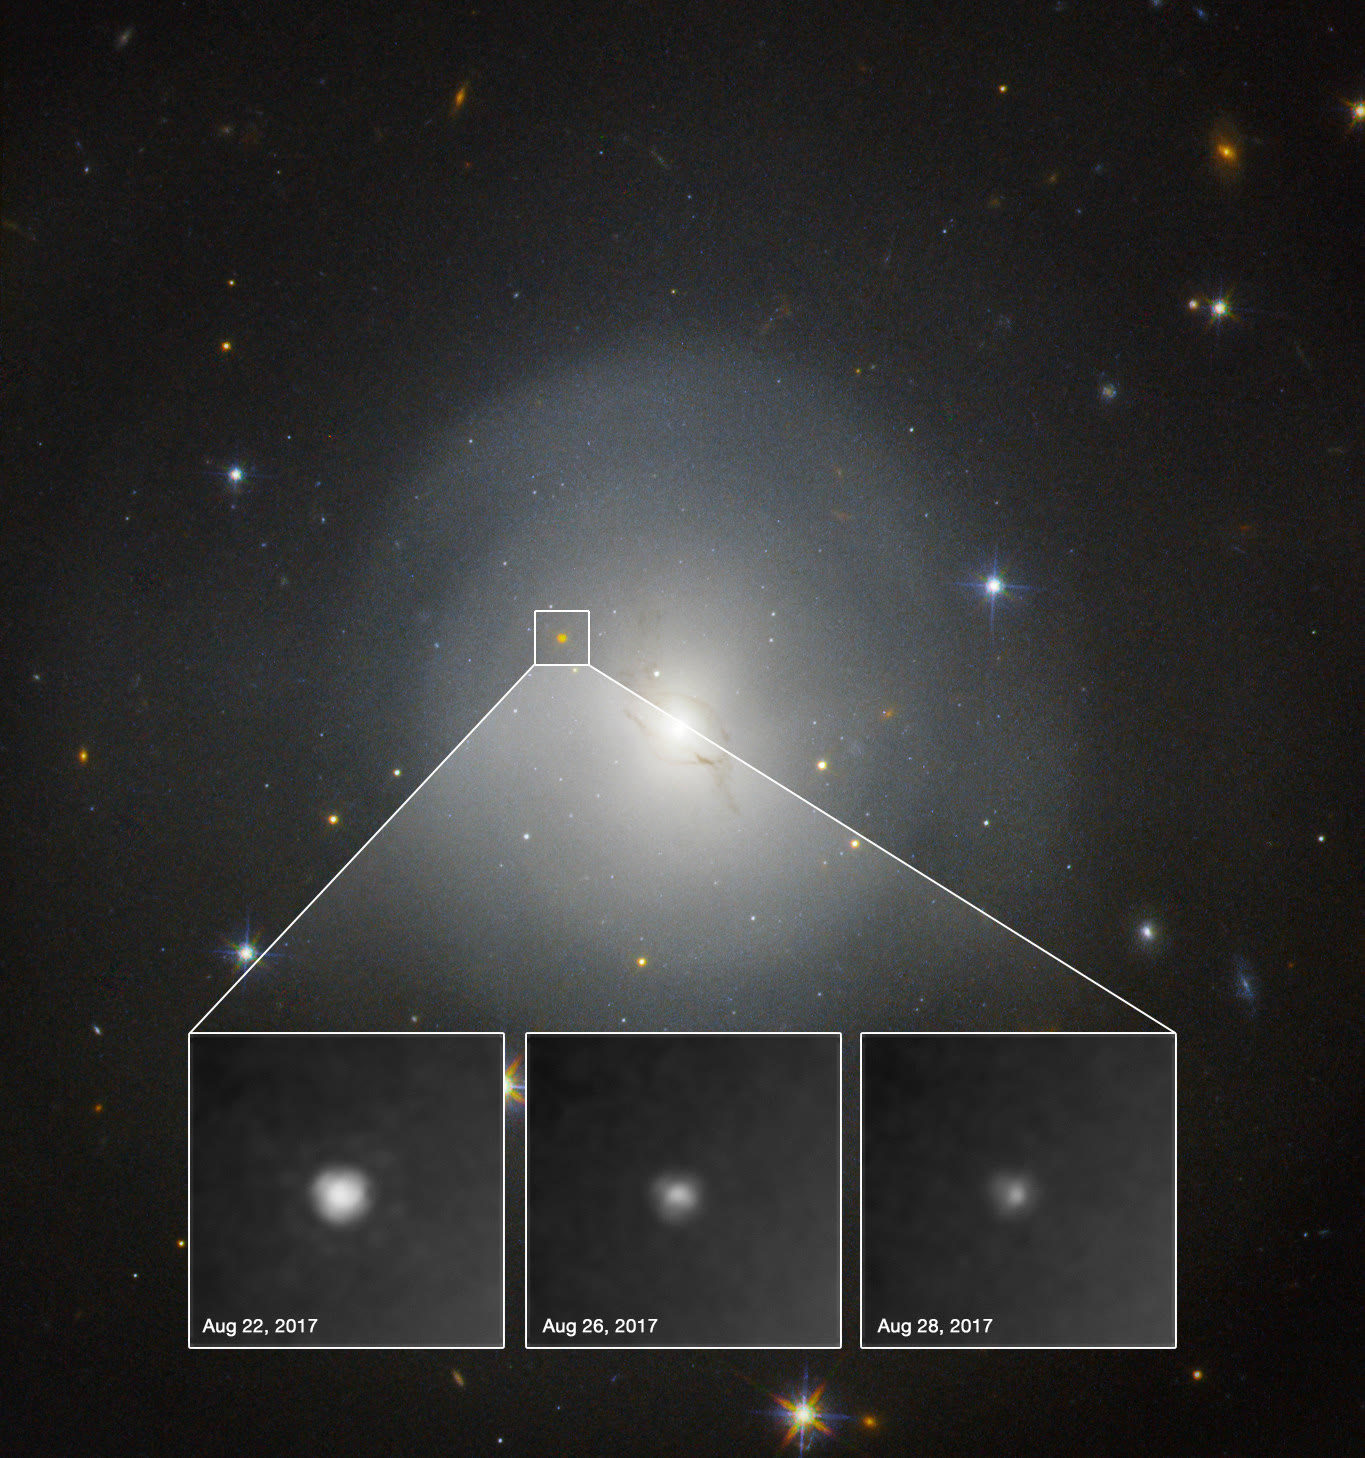
\includegraphics[width=0.55\linewidth]{images/book5/b3-kilonova.jpg}
\par\smallskip{\small المجرّة \babelsublr{NGC~4993} كما صوّرها تلسكوب هابل الفضائي
بعد اندماج نجمين نيوترونيين رُصد في
الموجات الثقالية في 17 آب 2017. يُحيط المربّع \omterm{def:b3:origin-of-elements:kilonova}{بالكيلونوفا}؛ أمّا
الإدراجات، المأخوذة في 22 و26 و28 آب، تُظهر خفوتها على مدى ستّة أيّام.
الصورة: \mbox{\textdir TLT NASA and ESA (A.~J.~Levan, N.~R.~Tanvir, A.~Fruchter and O.~Fox), CC BY~4.0}.
}\label{fig:b3:origin-of-elements:kilonova}
\end{omfigure}
% ledger: photo:b3-kilonova

\begin{dated}{2021}
لم يُحسم بعد ما إذا كانت اندماجات النجوم النيوترونية تصنع معظم عناصر \omterm{def:b3:origin-of-elements:s-process}{العملية r}
في المجرّة. فالاندماجات تنتظر انحلال مداراتها الثنائية،
والنماذج التي تجعلها المصدر الوحيد لتطوّر المجرّة
تُنتج عناصر \omterm{def:b3:origin-of-elements:s-process}{العملية r} متأخّرةً أكثر من اللازم لتفسير ما يُرصد في
أقدم النجوم وأفقرها بالمعادن. وأنواع نادرة من المستعرات العظمى ذات الانهيار القلبي،
ذات الدوران السريع والمجالات المغناطيسية القوية، وانهيار النجوم
الضخمة جدًّا هي المرشّحات الأخرى؛ ويفسّر أحد نماذج المجرّة
وفرة الأوروبيوم المرصودة إذا كانت نحو ثلاثة في المئة من
المستعرات الفائقة ذات الكتلة من 25 إلى \qty{50}{M_\odot} هي من النوع
المحرَّك مغناطيسيًّا.
\end{dated}
% ledger: kobayashi20:origins, cowan21:rprocess

\section{التطوّر الكيميائي للمجرّة}\label{sec:b3:origin-of-elements:gce}

يُعيد كلّ جيل من النجوم إلى الغاز بعضًا مما صنعه،
ويتكوّن الجيل التالي من ذلك الغاز المُثرى. ولذلك يسجّل تركيبُ النجم
تركيبَ الغاز عند ولادته، وتسجّل النجوم في المجرّة، مرتّبةً بحسب أعمارها،
تاريخَها.

\begin{definition}[التطوّر الكيميائي المجرّي]\label{def:b3:origin-of-elements:gce}
\emph{التطوّر الكيميائي المجرّي}\index{التطوّر الكيميائي المجرّي}
هو تغيّر تركيب الغاز والنجوم في مجرّة
مع الزمن، تحت الأثر المشترك لتكوين النجوم،
\omterm{def:b3:origin-of-elements:yield}{والمردود النجمي}، وأعمار النجوم، والغاز الذي يتدفّق إلى
المجرّة أو يُطرد منها؛ ودراسةُ ذلك التغيّر بنماذج
تُقارَن بوفرات النجوم المعلومة الأعمار.
\end{definition}
% ledger: matteucci21:simple

يعامل أبسط نموذج منطقةً من المجرّة بوصفها صندوقًا واحدًا جيّد الخلط من
الغاز يتحوّل ببطء إلى نجوم. ليكن $s$ كتلةَ المادة المحتجزة في
النجوم طويلة العمر وفي البقايا النجمية، و$M_\mathrm{g}$ كتلة الغاز،
و$M = M_\mathrm{g} + s$ الكتلة الكلّية. أمّا \emph{المردود لكلّ جيل
نجمي} $y$ فهو كتلة المعادن الجديدة التي يُعيدها جيل من النجوم
إلى الغاز لكلّ وحدة كتلة يحتجزها.
% ledger: matteucci21:yield

\begin{theorem}[نموذج الصندوق المغلق]\label{thm:b3:origin-of-elements:closed-box}
\index{نموذج الصندوق المغلق}
لنعتبر منطقةً لا تتبادل غازًا مع محيطها، تبدأ
غازًا نقيًّا خاليًا من المعادن، تبقى جيّدة الخلط، وفيها تموت النجوم
التي تصنع المعادن فورًا بينما تعيش الأخرى إلى الأبد (إعادة
التدوير اللحظية). فتكون معادنية الغاز
\[
Z = y \ln\frac{1}{\mu}, \qquad \mu = \frac{M_\mathrm{g}}{M},
\]
حيث $\mu$ نسبة الغاز، وكتلة النجوم المتكوّنة بمعادنية
أدنى من $Z$ هي \mbox{$M\,(1 - \mathrm{e}^{-Z/y})$}.
\end{theorem}

\begin{proof}
عندما تُحتجَز كتلة $\mathrm{d}s$ في النجوم، يفقد الغاز
$\mathrm{d}s$، مع المعادن التي يحتويها، $Z\,\mathrm{d}s$،
ويكتسب $y\,\mathrm{d}s$ من المعادن الجديدة:
$\mathrm{d}M_\mathrm{g} = -\mathrm{d}s$
و$\mathrm{d}(Z M_\mathrm{g}) = (y - Z)\,\mathrm{d}s$. وبنشر
المعادلة الثانية، $M_\mathrm{g}\,\mathrm{d}Z + Z\,\mathrm{d}M_\mathrm{g} =
y\,\mathrm{d}s - Z\,\mathrm{d}s$، فتتلاشى الحدود التي تحوي $Z$:
$M_\mathrm{g}\,\mathrm{d}Z = -y\,\mathrm{d}M_\mathrm{g}$. بالتكامل
من $M_\mathrm{g} = M$، $Z = 0$ يُعطي $Z = y\ln(M/M_\mathrm{g})$. أمّا
النجوم المتكوّنة بينما كانت معادنية الغاز أدنى من $Z$ فهي التي تكوّنت
حين انخفضت كتلة الغاز من $M$ إلى $M\mathrm{e}^{-Z/y}$، أي كتلةً
قدرها $M(1 - \mathrm{e}^{-Z/y})$.
\end{proof}
% ledger: matteucci21:simple

يتنبّأ النموذج بتوزيع المعادنية للنجوم طويلة العمر.
في الجوار الشمسي تبلغ الكثافة السطحية للغاز
\qty{13.7}{M_\odot.pc^{-2}}، وللنجوم والبقايا النجمية
\qty{33.4}{M_\odot.pc^{-2}}، ومنه $\mu = 13.7/47.1 = 0.29$. إذا كان الغاز
اليوم المعادنيةَ الشمسيةَ الأولى $Z = 0.0154$، فإنّ المردود
$y = 0.0154/\ln(1/0.29) = 0.0125$، وتكون نسبة جميع النجوم
المتكوّنة حتى الآن التي يكون فيها $Z$ أدنى من عُشر القيمة الحالية،
أي $[\mathrm{Fe/H}] < -1$ إن تبع الحديدُ المعادنَ، فتساوي
$(1 - 0.29^{0.1})/(1 - 0.29) = 0.16$.
% ledger: mckee15:surface, asplund21:xyz, data:b5-gce

\begin{omfigure}
\centering
\begin{tikzpicture}
\begin{axis}[width=0.95\linewidth, height=7.2cm, xmin=-1.6, xmax=0.7,
  ymin=0, ymax=1500, xlabel={$[\mathrm{Fe/H}]$},
  ylabel={عدد النجوم لكلّ \babelsublr{\num{0.1}~dex}},
  tick label style={font=\scriptsize}, label style={font=\small},
  legend style={font=\scriptsize, at={(0.5,-0.17)}, anchor=north,
    legend columns=3, draw=none, cells={anchor=west},
    /tikz/every even column/.append style={column sep=1em}}]
\addplot[ybar, area legend, bar width=0.085, fill=black!25, draw=black!50, bar shift=0pt]
  table[x=feh, y=n_obs] {figdata/out/bachelor-3-chemical_evolution-mdf.dat};
\addlegendentry{\foreignlanguage{arabic}{أقزام \mbox{\textdir TLT F} و\mbox{\textdir TLT G} (\mbox{\textdir TLT 6670})}}
\addplot[ybar, area legend, bar width=0.085, fill=blue!55, draw=blue!70!black, bar shift=0pt]
  table[x=feh, y=n_low] {figdata/out/bachelor-3-chemical_evolution-mdf.dat};
\addlegendentry{\foreignlanguage{arabic}{لا تتجاوز \qty{1}{M_\odot} (\mbox{\textdir TLT 902})}}
\addplot[red!75!black, very thick, const plot mark mid]
  table[x=feh, y=model] {figdata/out/bachelor-3-chemical_evolution-mdf.dat};
\addlegendentry{الصندوق المغلق}
\draw[black!50, dashed] (axis cs:-1,0) -- (axis cs:-1,1500);
\node[font=\scriptsize, anchor=north west, align=left] at (axis cs:-1.57,1450)
  {\foreignlanguage{arabic}{الصندوق المغلق: \mbox{\textdir TLT \qty{16}{\percent}}}\\\foreignlanguage{arabic}{تحت \mbox{\textdir TLT $-1$}؛}\\\foreignlanguage{arabic}{المرصود: \mbox{\textdir TLT \qty{0.4}{\percent}}}};
\end{axis}
\end{tikzpicture}
\par\smallskip{\small \omterm{def:b3:origin-of-elements:g-dwarf}{مسألة الأقزام G}. الأعمدة: معادنية الأقزام F و G
في الجوار الشمسي (\babelsublr{Geneva--Copenhagen survey}،
عيّنة أفضل القياسات الضوئية التي أعاد تحليلها كازاغراندي وآخرون،
2011)، جميع النجوم باللون الرمادي، وتلك التي لا تزيد كتلتها على كتلة شمسية واحدة، والنجوم طويلة العمر
التي يحسبها النموذج، باللون الأزرق. الخط: الصندوق المغلق
بنسبة الغاز الحالية في الجوار الشمسي، مُعايَر على
العدد نفسه من النجوم؛ ولا ينتج أيّ نجم أغنى من غازه الحالي،
المفترَض شمسيًّا. ويتنبّأ الصندوق بذيل طويل من النجوم
فقيرة بالمعادن لا وجود لها.}\label{fig:b3:origin-of-elements:g-dwarf}
\end{omfigure}
% ledger: data:b5-gcs, casagrande11:gcs, data:b5-gce, mckee15:surface

\begin{definition}[مسألة الأقزام G]\label{def:b3:origin-of-elements:g-dwarf}
\emph{مسألة الأقزام G}\index{مسألة الأقزام G} هي ندرة
النجوم الفقيرة بالمعادن الطويلة العمر في الجوار الشمسي مقارنةً بتنبّؤ
\omterm{thm:b3:origin-of-elements:closed-box}{نموذج الصندوق المغلق}: إذ تكون النجوم القزمة الطويلة العمر
من النمط الطيفي G ذات \omterm{def:b3:origin-of-elements:metallicity}{المعدنية} المنخفضة أقلّ بكثير مما يُفترض أن ينتجه
صندوق مغلق.
\end{definition}
% ledger: matteucci21:simple

من بين 6670 نجمًا في عيّنة المسح، لدى 26 منها $[\mathrm{Fe/H}] < -1$:
\qty{0.4}{\percent}، مقابل \qty{16}{\percent} في الصندوق المغلق.
حتى بين 902 نجمًا لا تزيد كتلتها على كتلة شمسية واحدة، وهي أعدل
مقارنة، تمثّل 26 نجمًا منها \qty{2.9}{\percent}. والمخرج هو فتح
الصندوق: فإذا بُني قرص الجوار الشمسي بسقوطٍ داخليٍّ بطيءٍ
للغاز الفقير بالمعادن على مدى عدّة مليارات من السنين، لم يكن الغاز الأوّلي قطّ
خزّانًا كبيرًا ينتظر تكوين نجوم فقيرة بالمعادن، ويختفي
الذيل. وتحتاج نماذج القرص التي تعيد إنتاج التوزيع إلى
زمن سقوط داخلي أطول من ثلاث إلى أربع مليارات سنة.
% ledger: data:b5-gcs, data:b5-gce, matteucci21:simple

الساعة الثانية هي نسبة نوعين من العناصر. وتأتي \omterm{def:b3:origin-of-elements:alpha}{عناصر
ألفا} من المستعرات العظمى بالانهيار اللبّي، بعيد ولادة جيل نجمي،
ويأتي جانب كبير من الحديد من المستعرات من النوع~Ia، بعد زمن طويل.
في نجوم الهالة القديمة، التي $[\mathrm{Fe/H}] < -1$،
تبلغ $[\alpha/\mathrm{Fe}]$ نحو $+0.4$: تكوّنت هذه النجوم من غاز
أُغني بالمستعرات العظمى بالانهيار اللبّي وحدها. وفي نجوم القرص تنخفض مع
ازدياد \omterm{def:b3:origin-of-elements:metallicity}{المعدنية} حتى الصفر، وهي القيمة الشمسية، مع إضافة
المستعرات من النوع~Ia حديدَها. ويُظهر الشكل أدناه أبسط نموذج
لهذه الصورة \emph{التأخّر الزمني}: ففي صندوق مغلق، يبدأ نوعا
المستعرات معًا، إلّا أنّ المستعرات من النوع~Ia تبدأ بعد تأخّرٍ ثابت
عن النجوم الأولى.
% ledger: matteucci21:time-delay, matteucci21:production

\begin{omfigure}
\centering
\begin{tikzpicture}
\begin{axis}[width=0.8\linewidth, height=6.4cm, xmin=-2.4, xmax=0.25,
  ymin=-0.08, ymax=0.55, xlabel={$[\mathrm{Fe/H}]$},
  ylabel={$[\alpha/\mathrm{Fe}]$},
  tick label style={font=\scriptsize}, label style={font=\small}]
\addplot[black!40, dashed, domain=-2.4:0.25, samples=2] {0};
\addplot[blue!70!black, very thick]
  table[x=feh, y=afe] {figdata/out/bachelor-3-chemical_evolution-alpha.dat};
\addplot[only marks, mark=*, mark size=2pt, red!70!black] coordinates {(-1,0.4) (0,0)};
\node[font=\scriptsize, anchor=south, align=center] at (axis cs:-1.75,0.41)
  {المستعرات العظمى بالانهيار اللبّي وحدها};
\node[font=\scriptsize, anchor=south west, align=left] at (axis cs:-0.98,0.41)
  {\foreignlanguage{arabic}{المستعرات من النوع Ia}\\[-1pt]\foreignlanguage{arabic}{تبدأ}};
\node[font=\scriptsize, anchor=south west] at (axis cs:0.01,0.01) {الشمس};
\end{axis}
\end{tikzpicture}
\par\smallskip{\small نموذج من مرحلتين للنسبة $[\alpha/\mathrm{Fe}]$ في
صندوق مغلق: الهضبة عند $+0.4$ هي النسبة التي تنتجها المستعرات
العظمى بالانهيار اللبّي؛ أمّا المستعرات من النوع~Ia، التي تبدأ حين يبلغ الغاز
$[\mathrm{Fe/H}] = -1$، فتضيف حديدًا بمعدّل ثابت، حتى تصبح النسبة
شمسية عند $[\mathrm{Fe/H}] = 0$. والهضبة والانعطاف هما ما يُرى في
نجوم درب التبانة؛ أمّا الشكل بينهما فهو من صنع النموذج.
عند معدنية الشمس، يكون \qty{60}{\percent} من الحديد في هذا النموذج
قد نشأ عن المستعرات من النوع~Ia.}\label{fig:b3:origin-of-elements:alpha}
\end{omfigure}
% ledger: data:b5-gce, matteucci21:time-delay

النماذج التفصيلية لدرب التبانة التي تُعيد إنتاج الاتجاه المرصود،
وتعزو ثلثي الحديد إلى المستعرات من النوع~Ia والثلث إلى
المستعرات العظمى بالانهيار اللبّي، وتجد أنّ غاز درب التبانة الفتيّة بلغ
$[\mathrm{Fe/H}] = -1$ في زمن يقارب من مليار إلى مليار ونصف من
السنين. والنسبة مِقياس زمني: \omterm{def:b3:milky-way-galaxies:populations}{فالجمهرة النجمية} الغنيّة \omterm{def:b3:origin-of-elements:alpha}{بعناصر ألفا}
عند معدنية معيّنة كوّنت نجومها بسرعة، قبل أن تستطيع المستعرات من النوع~Ia
إضافة حديدها. \omterm{def:b3:milky-way-galaxies:structure}{والقرص السميك} في
الفصل السابق هو مثل هذه الجمهرة: قديم، وغني قليلًا \omterm{def:b3:origin-of-elements:alpha}{بعناصر ألفا}
مقارنةً بنجوم القرص الرقيق ذات \omterm{def:b3:origin-of-elements:metallicity}{المعدنية} نفسها.
% ledger: matteucci21:time-delay, casagrande11:gcs

\section{من الوفرة الشمسية إلى الأرض}\label{sec:b3:origin-of-elements:earth}

تتكوّن الأرض من المادّة نفسها التي تتكوّن منها الشمس، لكن ليس من
كلّها. ففي السديم المتبرّد لم تُجمع إلّا العناصر التي تكثّفت صلبةً
في الكويكبات الأوّلية، وقد تتبّع مجلد السنة الثانية تسلسل تكثّفها.
يتكثّف الحديد معدنًا عند
نحو الدرجة نفسها التي تتكثّف عندها سيليكات المغنيسيوم، \qtyrange{1310}{1340}{K} عند
\qty{e-4}{bar}، لذا احتفظت الكواكب الصخرية بنصيبها من الحديد، بينما
بقيت الهيدروجين والهيليوم والكربون والنيتروجين والغازات النبيلة في الغاز.
من غاز ذي تركيب شمسي، لا يتكثّف إلّا نحو نصف في المئة من الكتلة
صخرًا ومعدنًا.
% ledger: lodders:tc-table, lodders:condensates

\begin{definition}[اتجاه التطاير]\label{def:b3:origin-of-elements:volatility}
\emph{اتجاه التطاير}\index{اتجاه التطاير} لجرمٍ كوكبي هو انخفاض وفرات عناصره
بالنسبة إلى كوندريتات CI، ومُطبَّعةً على عنصر صامد للحرارة،
مع انخفاض درجة حرارة التكاثف:
تبقى العناصر الصامدة بنسبها الكوندريتية،
بينما تنضب العناصر المتطايرة باعتدال كلّما انخفضت
درجة حرارة تكاثفها.
\end{definition}

بالنسبة إلى الأرض السيليكاتية، رسم مجلد السنة الثانية الاتجاه مقابل
درجة حرارة التكاثف. وبعد التطبيع على المغنيسيوم، يبلغ الزركونيوم
(الذي يتكثّف عند \qty{1741}{K}) يبلغ \num{1.11} مرّة نسبته في الكوندريتات
CI، والصوديوم (\qty{958}{K}) عند \num{0.22}، والبوتاسيوم
(\qty{1006}{K}) عند \num{0.19}، والروبيديوم (\qty{800}{K}) عند \num{0.12}
والزنك (\qty{726}{K}) عند \num{0.075}. وتكوّنت الأرض من مادّة
كانت قد فقدت جزءًا من عناصرها المتطايرة باعتدال قبل أن يكتمل تجمّع الكوكب،
أو فقدتها أثناء نموّه. وحتى كوندريتات CI تختلف عن الشمس
بطريقة تتبع درجة حرارة التكاثف، وإن كان ذلك بخفوت:
فعناصرها المتطايرة باعتدال تبلغ
نحو \num{0.04}~\omterm{def:b3:origin-of-elements:abundance}{dex} أعلى من القيم الضوئية.
% ledger: lodders:tc-table, lodders:ci-table, ms95:pm-trace, asplund21:abstract

وهكذا يمرّ سجلّ هذا الفصل عبر الكوكب. فالأكسجين
والمغنيسيوم والسيليكون في الوشاح \omterm{def:b3:origin-of-elements:alpha}{عناصر ألفا} قادمة من النجوم
الضخمة؛ أمّا حديد اللبّ فجاء في معظمه من المستعرات من النوع~Ia؛
والثوريوم واليورانيوم، اللذان يسهم تفكّكهما في تسخين الداخل، يقعان بعد
البزموث، حيث لا تصل إلّا \omterm{def:b3:origin-of-elements:s-process}{العملية r}؛ وخضع المزيج كلّه
لفرزٍ بحسب التطاير قبل أن تجمعه الأرض.
% ledger: matteucci21:production, matteucci21:time-delay, kaeppeler11:overview, data:b5-sigman

\section{التمارين}

\begin{exercise}[$\star$]\label{exo:b3:origin-of-elements:1}
باستعمال الوفرات الشمسية $\log\varepsilon(\mathrm{O}) = 8.69$،
$\log\varepsilon(\mathrm{Si}) = 7.51$، $\log\varepsilon(\mathrm{Fe}) =
7.46$، $\log\varepsilon(\mathrm{Au}) = 0.91$
و$\log\varepsilon(\mathrm{Pb}) = 1.95$: (أ)~كم ذرّة من السيليكون
وكم ذرّة من الأكسجين توجد في الشمس لكلّ ذرّة حديد؟ (ب)~كم
ذرّة حديد لكلّ ذرّة ذهب، وكم ذرّة رصاص لكلّ ذرّة ذهب؟
\end{exercise}

\begin{exercise}[$\star$]\label{exo:b3:origin-of-elements:2}
(أ)~كم ذرّة حديد لكلّ مليون ذرّة هيدروجين تحتوي عليها الشمس
($\log\varepsilon(\mathrm{Fe}) = 7.46$)؟ (ب)~لنجم من الهالة له
$[\mathrm{Fe/H}] = -2$. كم ذرّة هيدروجين يحتوي عليها لكلّ
ذرّة حديد؟ (ج)~نجم آخر فيه ذرّة حديد واحدة لكلّ عشرة ملايين
ذرّة هيدروجين. ما قيمة $[\mathrm{Fe/H}]$ له؟
\end{exercise}

\begin{exercise}[$\star$]\label{exo:b3:origin-of-elements:3}
للنظائر المستقرّة للزينون أعداد كتلية 124، 126، 128، 129، 130،
131، 132، 134 و136. ومن بين الكظيمات، للتيلوريوم ($Z = 52$)
نظائر مستقرّة هي 120، 122--126، 128 و130؛ أمّا الأيودين ($Z = 53$) فله 127 وحده.
يصل مسار s إلى الزينون عند $^{128}\mathrm{Xe}$، بتفكّك
$^{128}\mathrm{I}$، ويغادره عند $^{133}\mathrm{Xe}$ الذي يتفكّك.
صنّف كلّ نظير للزينون بأنّه s فقط، أو r فقط، أو مُنتَج بالعمليتين، أو
نواة p.
\end{exercise}

\begin{exercise}[$\star$]\label{exo:b3:origin-of-elements:4}
يقع GW170817 على بُعد نحو \qty{40}{Mpc}، ووصلت أشعّة غاما الصادرة عنه
بعد \qty{1.7}{s} من الاندماج المرصود بموجات الجاذبية. (أ)~كم من الزمن
سارت الإشارتان؟ (ب)~إذا نُسب التأخّر كلّه إلى
فرقٍ بين السرعتين، فكم يبلغ هذا الفرق بوصفه كسرًا
من سرعة الضوء على الأكثر؟
\end{exercise}

\begin{exercise}[$\star\star$]\label{exo:b3:origin-of-elements:5}
للنظائر الثلاثة s فقط للتيلوريوم وفرات ما قبل شمسية
\num{0.1067}، \num{0.0373} و\num{0.1984} لكلّ $10^6$ ذرّة سيليكون
($A = 122$، $123$، $124$) ومقاطع انتثار متوسّطة \num{295}،
\num{832} و\qty{155}{mb}. (أ)~احسب $\sigma N$ لكلّ منها. (ب)~انطلاقًا من
$^{122}\mathrm{Te}$ وحده، توقّع وفرات $^{123}\mathrm{Te}$
و$^{124}\mathrm{Te}$، وقارن بينهما. (ج)~لماذا لا يمكن تطبيق العلاقة
على $^{128}\mathrm{Te}$؟
\end{exercise}

\begin{exercise}[$\star\star$]\label{exo:b3:origin-of-elements:6}
في النموذج الكلاسيكي، تنقل كلّ نواة على مسار s إلى
النواة التالية كسرًا $f = 1/(1 + 1/(\tau_0\langle\sigma\rangle))$ من
الدفق، مع $\tau_0 = \qty{0.306}{mb^{-1}}$. (أ)~احسب $f$ من أجل
$^{124}\mathrm{Te}$ (\qty{155}{mb}) وللنواة السحرية بالنيوترونات
$^{138}\mathrm{Ba}$ (\qty{4.0}{mb}). (ب)~النوى الممتدّة من
$^{137}\mathrm{Ba}$ إلى $^{142}\mathrm{Nd}$ على المسار لها مقاطع عرضية
\num{76.3}، \num{4.0}، \num{32.4}، \num{11.0}،
\num{111.4} و\qty{35.0}{mb}. بأيّ عامل ينخفض $\sigma N$ من
$^{136}\mathrm{Ba}$ إلى $^{142}\mathrm{Nd}$؟ (ج)~قارن بالقيم
المقاسة \num{27.6} و\qty{7.72}{mb}.
\end{exercise}

\begin{exercise}[$\star\star$]\label{exo:b3:origin-of-elements:7}
لنيوترونٍ ذي الطاقة الحرارية $kT$ السرعةُ
$v_T = \sqrt{2kT/m_\mathrm{n}}$، حيث $m_\mathrm{n} = \qty{1.6749e-27}{kg}$.
(أ)~احسب $v_T$ عند $kT = \qty{8}{keV}$، وهي درجة حرارة
طبقة الكربون-13 في العملاق الأحمر. (ب)~بالنسبة إلى $^{124}\mathrm{Te}$، مع
$\langle\sigma\rangle = \qty{155}{mb}$، احسب متوسّط الزمن بين
أسرين متتاليين، $1/(n_\mathrm{n}\langle\sigma\rangle v_T)$، من أجل
$n_\mathrm{n} = 10^6$، $10^8$ و\qty{e10}{cm^{-3}}. (ج)~قارن بأعمار النصف لكلٍّ من
$^{127}\mathrm{Te}$ (\qty{9.35}{h})
و$^{134}\mathrm{Cs}$ (\qty{2.07}{yr}). أيّهما نقطة تفرّع؟
\end{exercise}

\begin{exercise}[$\star\star$]\label{exo:b3:origin-of-elements:8}
في الشمس، $\log\varepsilon$ يساوي \num{6.30} للكالسيوم، و\num{3.14}
للسكانديوم، و\num{4.97} للتيتانيوم؛ و\num{1.38} للبريليوم،
و\num{2.70} للبورون و\num{8.46} للكربون. (أ)~كم مرّة يكون السكانديوم أندر
من جاريه؟ (ب)~كم مرّة يكون
البريليوم أندر من الكربون؟ (ج)~أيّ سمة لمنحنى الوفرة تبيّنها
كلٌّ منها، وما سببها؟
\end{exercise}

\begin{exercise}[$\star\star$]\label{exo:b3:origin-of-elements:9}
في نموذج الطورين الوارد في الفصل، الهضبة
$[\alpha/\mathrm{Fe}] = P$ هي النسبة التي تنتجها المستعرات الأعظم ذات انهيار اللبّ،
وعند $[\mathrm{Fe/H}] = 0$ تكون النسبة شمسية. (أ)~بيّن أنّ حصّة
الحديد الشمسي المنتَج بالمستعرات الأعظم من النوع~Ia هي $1 - 10^{-P}$،
واحسب ذلك من أجل $P = 0.4$. (ب)~أيّ هضبة تعطي ثلثي
النماذج المفصّلة؟ (ج)~تُظهر مجرّة قزمة نقطة انحنائها عند
$[\mathrm{Fe/H}] = -2$. ماذا يخبرنا ذلك عن تكوّن نجومها؟
\end{exercise}

\begin{exercise}[$\star\star\star$]\label{exo:b3:origin-of-elements:10}
تحتوي كوندريتات CI، بأجزاء في المليون بالكتلة، على \num{95870}
من المغنيسيوم، و\num{3.96} من الزركونيوم، و\num{5010} من الصوديوم، و\num{530}
من البوتاسيوم، و\num{2.13} من الروبيديوم؛ بينما تحتوي الأرض السيليكاتية على
\qty{22.8}{\percent} من المغنيسيوم، و\num{10.5}، \num{2670}، \num{240}
و\num{0.6} جزءًا في المليون من العناصر الأخرى. ودرجات حرارة التكاثف عند 50~في المئة
هي \qty{1336}{K} للمغنيسيوم \babelsublr{(Mg)}، \qty{1741}{K} للزركونيوم \babelsublr{(Zr)}،
\qty{958}{K} للصوديوم \babelsublr{(Na)}، \qty{1006}{K} للبوتاسيوم \babelsublr{(K)} و\qty{800}{K} للروبيديوم \babelsublr{(Rb)}. (أ)~من أجل
كلّ عنصر، احسب $(X/\mathrm{Mg})_\mathrm{Earth}/(X/\mathrm{Mg})_\mathrm{CI}$.
(ب)~ارسمها بدلالة درجة حرارة التكاثف، وصِف
الاتجاه. (ج)~لماذا يُختار المغنيسيوم مرجعًا؟
\end{exercise}

\begin{exercise}[$\star\star\star$]\label{exo:b3:origin-of-elements:11}
يفقد الصندوق المتسرّب غازًا في ريح بمعدّل $\lambda$ مضروبًا في معدّل
تكوّن النجوم، ولا يستقبل أيّ غاز. (أ)~بيّن أنّ \omterm{def:b3:origin-of-elements:metallicity}{المعدنية} فيه هي
$Z = \frac{y}{1 + \lambda}\ln\frac{M_\mathrm{g}(0)}{M_\mathrm{g}}$.
(ب)~مع $y = 0.0125$، قارن \omterm{def:b3:origin-of-elements:metallicity}{المعدنية} المبلوغة حين يصبح الغاز قد
هبط إلى \qty{29}{\percent} من كتلته الأولية، من أجل $\lambda = 0$
و$\lambda = 1$. (ج)~لماذا تميل المجرّات الصغيرة، ذات الجاذبية الضعيفة، إلى أن تكون
فقيرة بالمعادن؟
\end{exercise}

\begin{exercise}[$\star\star\star$]\label{exo:b3:origin-of-elements:12}
(أ)~تحتوي الشمس على $\log\varepsilon(\mathrm{Li}) = 0.96$ في غلافها الضوئي، والكوندريتات CI على $3.25$. احسب النسبتين $N_\mathrm{Li}/N_\mathrm{H}$
وكسر الليثيوم الذي دمّرته الشمس منه. (ب)~أقدم
النجوم الفقيرة بالمعادن تُظهر $N_\mathrm{Li}/N_\mathrm{H} = \num{1.45e-10}$،
بينما يتنبّأ التخليق النووي للانفجار الكبير بالقيمة \num{4.72e-10}. بأيّ عامل
يتجاوز ليثيوم المجموعة الشمسية كلًّا منهما؟ (ج)~ماذا
تستلزم
المقارنتان؟
\end{exercise}

\section{مسألة: مجرّة الصندوق المغلق}

\begin{problem}[{مسألة نهاية الأسبوع --- من خليط الشمس إلى
معدنيات النجوم طويلة العمر}]
\label{pb:b3:origin-of-elements:1}
استخدم $\log\varepsilon(\mathrm{H}) = 12$، والوفرات الشمسية
$\log\varepsilon(\mathrm{Fe}) = 7.46$، و$\log\varepsilon(\mathrm{O}) =
8.69$، و$\log\varepsilon(\mathrm{He}) = 10.914$، والكسور الكتلية الضوئية الحالية
$X = 0.7438$، و$Y = 0.2423$، و$Z = 0.0139$،
و$Z_\odot = 0.0154$ للسديم الشمسي الأوّلي. افترض في كلّ ما يلي أنّ الحديد
يتبع \omterm{def:b3:origin-of-elements:metallicity}{المعدنية} الكلّية، $[\mathrm{Fe/H}] = \log_{10}(Z/Z_\odot)$.

\medskip\noindent\textbf{الجزء الأول --- خليط الشمس.}
\begin{enumerate}
\item كم ذرّة هيدروجين توجد في الشمس لكلّ ذرّة حديد؟
\item احسب نسبة الأعداد $N_\mathrm{He}/N_\mathrm{H}$. مع اعتبار
  ذرّة الهيليوم أثقل من ذرّة الهيدروجين أربع مرّات، قارن
  $4N_\mathrm{He}/N_\mathrm{H}$ مع $Y/X$.
\item تحتوي نجمة على ذرّة حديد واحدة لكلّ \num{350000} ذرّة هيدروجين.
  احسب $[\mathrm{Fe/H}]$ لها إلى رقمين عشريين.
\item للنجمة نفسها $[\mathrm{O/Fe}] = +0.40$. احسب
  $\log\varepsilon(\mathrm{O})$ لها، وعدد ذرّات الأكسجين لكلّ ذرّة حديد
  مقارنةً بالشمس.
\item الأكسجين هو أوفر المعادن. قدّر كسر الكتلة \omterm{def:b3:origin-of-elements:metallicity}{المعدنية} للنجمة
  بتحجيم كسر الشمس بحسب $[\mathrm{O/H}]$.
\item لماذا تُقاس معدنية النجمة عادةً من الحديد
  لا من الأكسجين، مع أنّ الأكسجين يهيمن على $Z$؟
\end{enumerate}

\medskip\noindent\textbf{الجزء الثاني --- عملية s على التيلوريوم.} استخدم
البيانات الواردة في \cref{exo:b3:origin-of-elements:5}.
\begin{enumerate}[resume]
\item اشرح من مخطط النويدات لماذا تكون $^{122}\mathrm{Te}$،
  $^{123}\mathrm{Te}$ و$^{124}\mathrm{Te}$ من نوع s فقط.
\item احسب $\sigma N$ للنظائر الثلاثة ومتوسطها.
\item تنبّأ بوفرة $^{123}\mathrm{Te}$ من متوسط
  النظيرين الآخرين، وأعطِ الفرق عن القيمة المقاسة بالنسبة
  المئوية.
\item لدى $^{128}\mathrm{Te}$ القيمة $N = 1.329$ لكلّ $10^6$ من Si
  و$\langle\sigma\rangle = \qty{44.4}{mb}$. احسب $\sigma N$ له، واذكر
  لماذا لا يقع على الهضبة.
\item الزوج $^{148}\mathrm{Sm}$ و$^{150}\mathrm{Sm}$ من نوع s فقط، ولديه
  $\sigma N = \num{7.43}$ و\qty{8.53}{mb}. ما حصّة التدفّق
  الذي مرّ حول $^{148}\mathrm{Sm}$، وعبر أيّ تفرّع؟
\item عبر $N = 82$ ينخفض الناتج من \qty{27.6}{mb}
  ($^{136}\mathrm{Ba}$) إلى \qty{7.72}{mb} ($^{142}\mathrm{Nd}$). أيّ
  خاصيّة للنويدات ذات $N = 82$ تفسّر الهبوط؟
\end{enumerate}

\medskip\noindent\textbf{الجزء الثالث --- الصندوق المغلق.} يحتوي جوار
الشمس على \qty{13.7}{M_\odot.pc^{-2}} من الغاز
و\qty{33.4}{M_\odot.pc^{-2}} من النجوم وبقاياها. افترض أنّ
الغاز الحالي يملك $Z = Z_\odot$.
\begin{enumerate}[resume]
\item احسب كسر الغاز الحالي $\mu_1$.
\item احسب الناتج لكلّ جيل نجمي $y$ الذي يحتاجه
  الصندوق المغلق، ونسبته إلى $Z_\odot$.
\item احسب $Z$ و$[\mathrm{Fe/H}]$ للغاز حين كان كسر الغاز
  $0.9$، ثم $0.5$.
\item احسب كسر الغاز حين بلغ الغاز
  $[\mathrm{Fe/H}] = -1$.
\item ما كسر الكتلة الكلّية الذي كان قد حُبس عندئذٍ في النجوم؟
\item لو كان كسر الغاز الحالي $0.1$ بدلًا من ذلك، فما الناتج الذي
  يحتاجه الصندوق؟
\end{enumerate}

\medskip\noindent\textbf{الجزء الرابع --- توزيع \omterm{def:b3:origin-of-elements:metallicity}{المعدنية}.}
\begin{enumerate}[resume]
\item بيّن أنّ الصندوق المغلق يعطي توزيعًا للنجوم في
  $[\mathrm{Fe/H}]$ يتناسب مع $Z\,\mathrm{e}^{-Z/y}$، وأوجد
  $[\mathrm{Fe/H}]$ عند قمّته.
\item احسب كسر جميع النجوم المتكوّنة حتى الآن ذات
  $[\mathrm{Fe/H}] < -1$.
\item احسب الكسر ذا $[\mathrm{Fe/H}] < -0.5$.
\item في عيّنة المسح المكوّنة من 6670 قزمًا من النوعين F وG، لدى 26 منها
  $[\mathrm{Fe/H}] < -1$. كم عددها يتنبّأ به الصندوق المغلق؟
\item من بين 902 نجمًا لا تتجاوز كتلته كتلة شمسية واحدة، يُرصد العدد نفسه،
  أي 26 نجمًا. احسب الكسر المرصود، واذكر لماذا تُعدّ هذه العيّنة الجزئية المقارنة الأعدل.
  المقارنة الأعدل.
\item مع كسر غاز حالي قدره $0.1$، ما الكسر المتنبّأ به
  تحت $-1$؟ هل يحلّ كسر غاز مختلف
  المشكلة؟
\item أعطِ كسر النجوم طويلة العمر ذات $[\mathrm{Fe/H}] < -1$
  الذي يتنبّأ به الصندوق المغلق لجوار الشمس، بالنسبة المئوية،
  برقمين معنويين، واذكر ما تعنيه المقارنة مع
  النجوم المرصودة لتاريخ القرص.
\end{enumerate}
\end{problem}
% ledger: asplund21:abstract, asplund21:xyz, data:b5-sigman, data:b5-kadonis, mckee15:surface, data:b5-gcs, data:b5-gce, matteucci21:simple
